\selectlanguage{italian}

\section{Radioattività}

I primi indizi verso la radioattività sono derivati dalla rilevazione dei raggi X: questi sono onde elettromagnetiche, ovvero fotoni, generate da transizioni di elettroni tra livelli energetici ($ \Delta E_e = \hbar \omega $); questi dunque non sono processi nucleari, dato che avvengono all'interno della nube elettronica dell'atomo.\\
Quando si parla di radioattività in senso stretto, però, si fa riferimento ai decadimenti dei nuclidi.

\subsection{Decadimenti radioattivi}

I decadimenti radioattivi sono processi in cui un nuclide instabile raggiunge una configurazione con energia più bassa emettendo spontaneamente radiazione.\\
Utilizzando un campo magnetico, Rutherford riuscì a distinguere tre tipologie di radiazione, e dunque di decadimenti radioattivi:
\begin{enumerate}
  \item decadimento $ \alpha $, in cui la radiazione è costituita da un nucleo di $ \ch{^4_2 He} $ ed è poco penetrante, coinvolge l'interazione elettromagnetica e quella forte;
  \item decadimento $ \beta^{\pm} $, in cui la radiazione è costituita da un $ e^{\pm} $ ed è mediamente penetrante, coinvolge l'interazione debole:
    \begin{itemize}
      \item decadimento $ \beta^- $: $ n \rightarrow p^+ + e^- + \bar{\nu}_e $;
      \item decadimento $ \beta^+ $: $ p^+ \rightarrow n + e^+ + \nu_e $;
    \end{itemize}
  \item decadimento $ \gamma $, in cui la radiazione è costituita da un fotone con energia dell'ordine delle decine di MeV, dunque estremamente penetrante.
\end{enumerate}
A questi si aggiunge la cattura elettronica, un decadimento in cui un nuclide proton-rich cattura un elettrone dalle shell interne dell'atomo, seguendo la reazione $ p^+ + e^- \rightarrow n + \nu_e $, emettendo raggi X a seguito del rimpiazzo dell'elettrone interno con uno dalle shell esterne.

\subsection{Energy balance}

Un decadimento radioattivo può essere visto come un caso particolare di reazione nucleare; è quindi possibile definire il $ Q $-value del decadimento come la differenza di energia a riposo (massa) tra reagenti (nuclide instabile) e prodotti, così da poter stabilire qualora esso sia possibile, ovvero spontaneo, con la condizione $ Q > 0 $.\\
In particolare, si definiscono i $ Q $-values dei seguenti decadimenti:
\begin{enumerate}
  \item decadimento $ \alpha $: $ Q_{\alpha} \equiv \left[ M(Z,A) - M(Z-2,A-4) - m(\ch{^4_2 He}) \right] c^2 $;
  \item decadimento $ \beta^- $: $ Q_{\beta^-} \equiv \left[ M(Z,A) - M(Z+1,A) - m_e \right] c^2 $;
  \item decadimento $ \beta^+ $: $ Q_{\beta^+} \equiv \left[ M(Z,A) - M(Z-1,A) - m_e \right] c^2 $;
  \item electron capture: $ Q_{e} \equiv \left[ M(Z,A) + m_e - M(Z-1,A) \right] c^2 $;
\end{enumerate}
Si vede subito che $ Q_e > Q_{\beta^+} $: di conseguenza, nell'electron capture i prodotti di decadimento hanno maggior energia cinetica disponibile, inoltre ci sono dei casi in cui può avvenire l'electron capture ma non il decadimento $ \beta^+ $.

\subsection{Radioactive decay law}

Il processo di decadimento ha natura aleatoria, dunque va trattato in maniera statistica.\\
Il numero di decadimenti al secondo è proporzionale al numero di nuclidi radioattivi:
\begin{equation}
	- \frac{dN}{dt} = \lambda N(t)
	\label{eq:2.1}
\end{equation}
Si trova quindi la legge di decadimento esponenziale:
\begin{equation}
	N(t) = N_0 e^{-\lambda t}
	\label{eq:2.2}
\end{equation}
Si definisce inoltre il decay rate (o activity) come $ A(t) \defeq \lambda N(t) $, misurato in Bequerel $ 1\,\text{Bq} = 1 \,\text{decay}/\text{s} $ o in Curie $ 1\,\text{Ci} = 3.7\cdot10^{10}\,\text{Bq} $ (activity di $ 1\,\text{g} $ di radio). Si definiscono inoltre la half-life $ t_{1/2} \equiv \frac{\ln 2}{\lambda} $ e la vita media $ \tau = \frac{1}{\lambda} $ rispettivamente come il tempo dopo il quale il campione si è ridotto di $ \frac{1}{2} $ e di $ \frac{1}{e} $: si ha $ t_{1/2} \approx 0.693 \tau < \tau $.\\
Per i decay rates si trova facilmente che, definendo $ A_0 \equiv \lambda N_0 $:
\begin{equation}
	A((n+1)t) = A(t) \left( \frac{A(t)}{A_0} \right)^n
	\label{eq:2.3}
\end{equation}
Nel caso di una miscela di radioisotopi, è possibile risalire alle singole costanti di decadimento nel caso in cui le vite medie siano molto diverse, poiché quando la specie con la $ \tau $ più corta è completamente decaduta si può misurare direttamente la $ \lambda $ dell'altra specie, per poi risalire a quella della prima tramite la differenza delle activities.

\subsubsection{Decay branches}

Può capitare che lo stesso nuclide radioattivo possa decadere in due o più modi differenti, detti decay branches: detta $ \lambda_k $ la costante di decadimento parziale della $ k $-esima branch, nel caso di $ n $ branches si ha:
\begin{equation}
	\lambda \equiv \lambda_1 + \dots + \lambda_n
	\label{eq:2.4}
\end{equation}
e questa costante totale è l'unica che si osserva, anche quando si rileva una sola delle branches. Si definiscono i branching ratios come $ B_k \defeq \frac{\lambda_k}{\lambda} $.

\subsubsection{Decay chains}

Spesso, in un decadimento radioattivo, capita che anche i prodotti siano radioattivi: ciò dà vita ad una catena di decadimenti $ N_1 \xrightarrow{\lambda_1} N_2 \xrightarrow{\lambda_2} N_3 \dots $, dove le $ \lambda_k $ sono diverse tra loro.\\
Una decay chain è descritto da un sistema di coupled differential equations. Nel caso, ad esempio, di un doppio decadimento (quindi con prodotto $ N_3 $ stabile):
\begin{equation}
	\begin{cases}
		\dot{N}_1 = - \lambda_1 N_1 \\
		\dot{N}_2 = \lambda_1 N_1 - \lambda_2 N_2 \\
		\dot{N}_3 = \lambda_2 N_2
	\end{cases}
	\quad\Longrightarrow\quad
	\begin{cases}
		N_1(t) = N_0 e^{-\lambda_1 t} \\
		N_2(t) = \frac{\lambda_1}{\lambda_1 + \lambda_2} N_0 \left( e^{-\lambda_1 t} - e^{-\lambda_2 t} \right) \\
		N_3(t) = \frac{\lambda_1 \lambda_2}{\lambda_1 + \lambda_2} N_0 \left( \frac{1 - e^{-\lambda_1 t}}{\lambda_1} - \frac{1 - e^{-\lambda_2 t}}{\lambda_2} \right)
	\end{cases}
	\label{eq:2.5}
\end{equation}
La soluzione generale al caso di $ n $ decadimenti è dato dall'\textit{equazione di Bateman}:
\begin{equation}
	N_k(t) = \sum_{i = 1}^{k} \left[ N_0^{(i)} \left( \prod_{j = 1}^{k-1} \lambda_j \right) \left( \sum_{j = i}^{k} \frac{e^{-\lambda_j t}}{\prod_{p=i, p\neq j}^{k} (\lambda_p - \lambda_j)} \right) \right]
	\label{eq:2.6}
\end{equation}

\paragraph{Equilibrio radioattivo} Si parla di equilibrio radioattivo quando la specie radioattiva madre e quella figlia hanno la stessa attività, ovverosia quando la specie figlia decade allo stesso rate a cui è prodotta. In una decay chain, l'equilibrio radioattivo può instaurarsi tra ciascuna coppia di nuclidi della catena: la condizione generale da soddisfarre è che $ (t_{1/2})_{\text{madre}} > (t_{1/2})_{\text{figlia}} $.\\
In particolare, si parla di:
\begin{enumerate}
	\item equilibrio transiente: si ha quando $ (t_{1/2})_{\text{madre}} \approx (t_{1/2})_{\text{figlia}} $, dunque, dopo un periodo di transienza iniziale, l'activity della specie madre e quella della specie figlia diventano uguali;
	\item equilibrio secolare: si ha quando $ (t_{1/2})_{\text{madre}} \rightarrow \infty $ (comparabile all'età della Terra), dunque la sua activity è praticamente costante; di conseguenza, dopo un certo periodo di tempo, anche l'activity della specie figlia diventerà costante e pari a quella della specie madre (si vede analiticamente dall'Eq. 2.5 ponendo $ \lambda_1 \ll \lambda_2 $). Si parla di equilibrio secolare anche quando, più genericamente, $ (t_{1/2})_{\text{madre}} \gg (t_{1/2})_{\text{figlia}} $.
\end{enumerate}

\paragraph{Serie radioattive naturali}

Ci sono 4 decay chains naturali principali, tutte composte da decadimenti $ \alpha $ e $ \beta^- $:
\begin{enumerate}
  \item serie del torio: inizia col $ \ch{^{232} Th} $ e termina col $ \ch{^{208} Pb} $, il decadimento col tempo di dimezzamento più lungo è $ \ch{^{232} Th} \rightarrow \ch{^{228} Ra} $ con $ t_{1/2} = 14 \,\text{Gy} $;
  \item serie dell'uranio: inizia col $ \ch{^{238} U} $ e termina col $ \ch{^{206} Pb} $, il decadimento col tempo di dimezzamento più lungo è $ \ch{^{238} U} \rightarrow \ch{^{234} Th} $ con $ t_{1/2} = 4.5 \,\text{Gy} $;
  \item serie del plutonio: inizia col $ \ch{^{239} Pu} $ e termina col $ \ch{^{207} Pb} $, il decadimento col tempo di dimezzamento più lungo è $ \ch{^{235} U} \rightarrow \ch{^{231} Th} $ con $ t_{1/2} = 0.71 \,\text{Gy} $;
  \item serie del nettunio: inizia col $ \ch{^{237} Np} $ e termina col $ \ch{^{209} Bi} $, il decadimento col tempo di dimezzamento più lungo è $ \ch{^{237} Np} \rightarrow \ch{^{233} Pa} $ con $ t_{1/2} = 2.3 \,\text{My} $;
\end{enumerate}
Quest'ultima serie non è più osservabile in natura poiché la sua vita media non è comparabile con l'età della Terra, a differenza delle altre tre.

\paragraph{Carbon dating}

Il $ \ch{^{14}C} $ è un isotopo radioattivo del carbonio con $ t_{1/2} = 5730\,\text{y} $; nonostante questa vita media relativamente corta, esso è prodotto continuamente grazie ai raggi cosmici in atmosfera tramite neutron capture: $ \ch{^{14}N} + n \rightarrow \ch{^{14}C} + p^+ $; una volta assorbito dai sistemi biologici, esso decade per decadimento $ \beta^- $: $ \ch{^{14}C} \rightarrow \ch{^{14}N} + e^- + \bar{\nu}_e $.\\
Misurata la specific activity $ a $ del campione da datare, si può risalire al time since death comparandola alla standard specific activity $ a_0 = 0.266\,\text{Bq}/\text{g} $: $ T = \frac{t_{1/2}}{\ln 2} \ln \frac{a}{a_0} = - 8033\,\text{y} \cdot \ln \frac{a}{a_0} $.\\
L'assunzione fondamentale di questo metodo di datazione è che la concentrazione naturale di $ \ch{^{14}C} $ rimanga costante nel tempo: con la Guerra Fredda questo è diventato un problema, poiché i test nucleari hanno fatto raddoppiare per un periodo tale concentrazione, e solo ultimamente si sta tornando ai livelli precedenti. Inoltre, l'aumento della combustione di combustibili fossili ha diluito l'atmosfera con carbonio stabile: gli idrocarburi, infatti, sono vecchi a sufficienza per aver esaurito la loro concentrazione di $ \ch{^{14}C} $. Infine, va notato che il carbon dating è efficace solo per oggetti non più vecchi di 50'000 anni: per epoche precedenti, sono necessari altre coppie isotopiche, come ad esempio $ \ch{^{40}K} $ - $ \ch{^{40}Ar} $, $ \ch{^{235}U} $ - $ \ch{^{207}Pb} $ o $ \ch{^{238}U} $ - $ \ch{^{208}Pb} $.

\section{Decadimento \texorpdfstring{$ \alpha $}{TEXT}}

Il decadimento $ \alpha $ consiste nell'emissione di un nucleo di $ \ch{^4 He} $ da parte di un nucleo instabile, secondo la reazione:
\begin{equation}
	\ch{^A_Z X_N} \rightarrow \ch{^{A-4}_{Z-2} Y_{N-2}} + \ch{^4_2 He_{2}}
	\label{eq:2.7}
\end{equation}
Questo avviene grazie alla repulsione coulombiana tra nucleo e $ \alpha $, espressa dall'andamento dell'energia potenziale:
\begin{equation}
	U(r) = \frac{2(Z-2)e^2}{4\pi \epsilon_0 r}
	\label{eq:2.8}
\end{equation}
È il decadimento prevalente nei nuclei pesanti: ad elevati $ A $ conviene ridurre la massa del sistema per acquisire maggiore stabilità (si veda Fig. \ref{bind-en}). Per lo stesso motivo, non si osservano decadimenti $ \alpha $ in nuclei più leggeri del $ \ch{^{126}_{62} Sm} $.

\paragraph{Bilancio energetico}

È fondamentale studiare il bilancio energetico del decadimento $ \alpha $: in particolare, esso è possibile quando il $ Q $-value dell'Eq. $ \ref{eq:2.7} $ è positivo. Assumendo che il nuclide instabile sia inizialmente a riposo:
\begin{equation}
	Q = T_{\ch{Y}} + T_{\alpha} = \left( m_{\ch{X}} - m_{\ch{Y}} - m_{\alpha} \right) c^2
	\label{eq:2.9}
\end{equation}
A ciò va aggiunta la conservazione del momento lineare, la quale impone che $ \ve{p}_{\ch{Y}} = -\ve{p}_{\alpha} $, con la quale si trova (trattando non-relativisticamente, dato che i valori tipici sono $ T_{\alpha} \sim 5\mev $):
\begin{equation}
	T_{\alpha} = \frac{m_{\ch{Y}}}{m_{\ch{Y}} + m_{\alpha}} Q \approx \left( 1 - \frac{4}{A} \right) Q
	\label{eq:2.10}
\end{equation}
Dunque $ \alpha $ trasporta circa il $ 98\% $ del $ Q $-value ($ \sim 5\mev $), mentre il restante $ 2\% $ ($ \sim 0.1\mev $) viene trasmesso al nuclide figlio $ \ch{Y} $ come recoil energy (può diventare significativa in decay chains, portando a radioactive material leaks).\\
Si osserva inoltre che, essendo il decadimento $ \alpha $ un decadimento a due corpi, le particelle emesse sono mono-energetiche, ovvero, fissata la specie nucleare che decade, le particelle $ \alpha $ vengono emesse tutte praticamente con la stessa energia fissata dall'Eq. \ref{eq:2.10}. Ciò non vale per i decadimenti a tre o più corpi.

\subsection{Systematics}

Osservazioni sperimentali (condotte originariamente da Geiger e Nuttall) rivelano che, sebbene il processo di decadimento sia fondamentalmente sempre lo stesso, i tempi di dimezzamento possono variare di svariati ordini di grandezza tra le varie specie nucleari, in relazione anche a come varia il $ Q $-value: si va dal $ \ch{^{232}Th} $ con $ t_{1/2} = 14 \,\text{Gy} $ e $ Q = 4.08\mev $ al $ \ch{^{218}Th} $ con $ t_{1/2} = 0.1 \,\mu\text{s} $ e $ Q = 9.85\mev $, ovvero una variazione di 24 ordini di grandezza nella half-life a fronte di un solo fattore 2 nel $ Q $-value.\\
Plottando i dati sperimentali (Fig. \ref{geiger-nuttall}) si osserva un trend che prende il nome di \textit{legge di Geiger-Nuttall}:
\begin{equation}
	\ln t_{1/2} = a(Z) + \frac{b(Z)}{\sqrt{Q}}
	\label{eq:2.11}
\end{equation}
dove $ a $ e $ b $ sono parametri empirici. La conferma teorica di questa legge è stata una delle prime prove della meccanica quantistica.\\
Studiando invece la dipendeza di $ Q $ da $ A $ (Fig. \ref{gn-mass}) si può osservare un'importante discontinuità in corrispondenza di $ N = 126 $, mostrando ancora una volta la presenza di una nuclear shell structure.

\begin{figure}
	\centering
	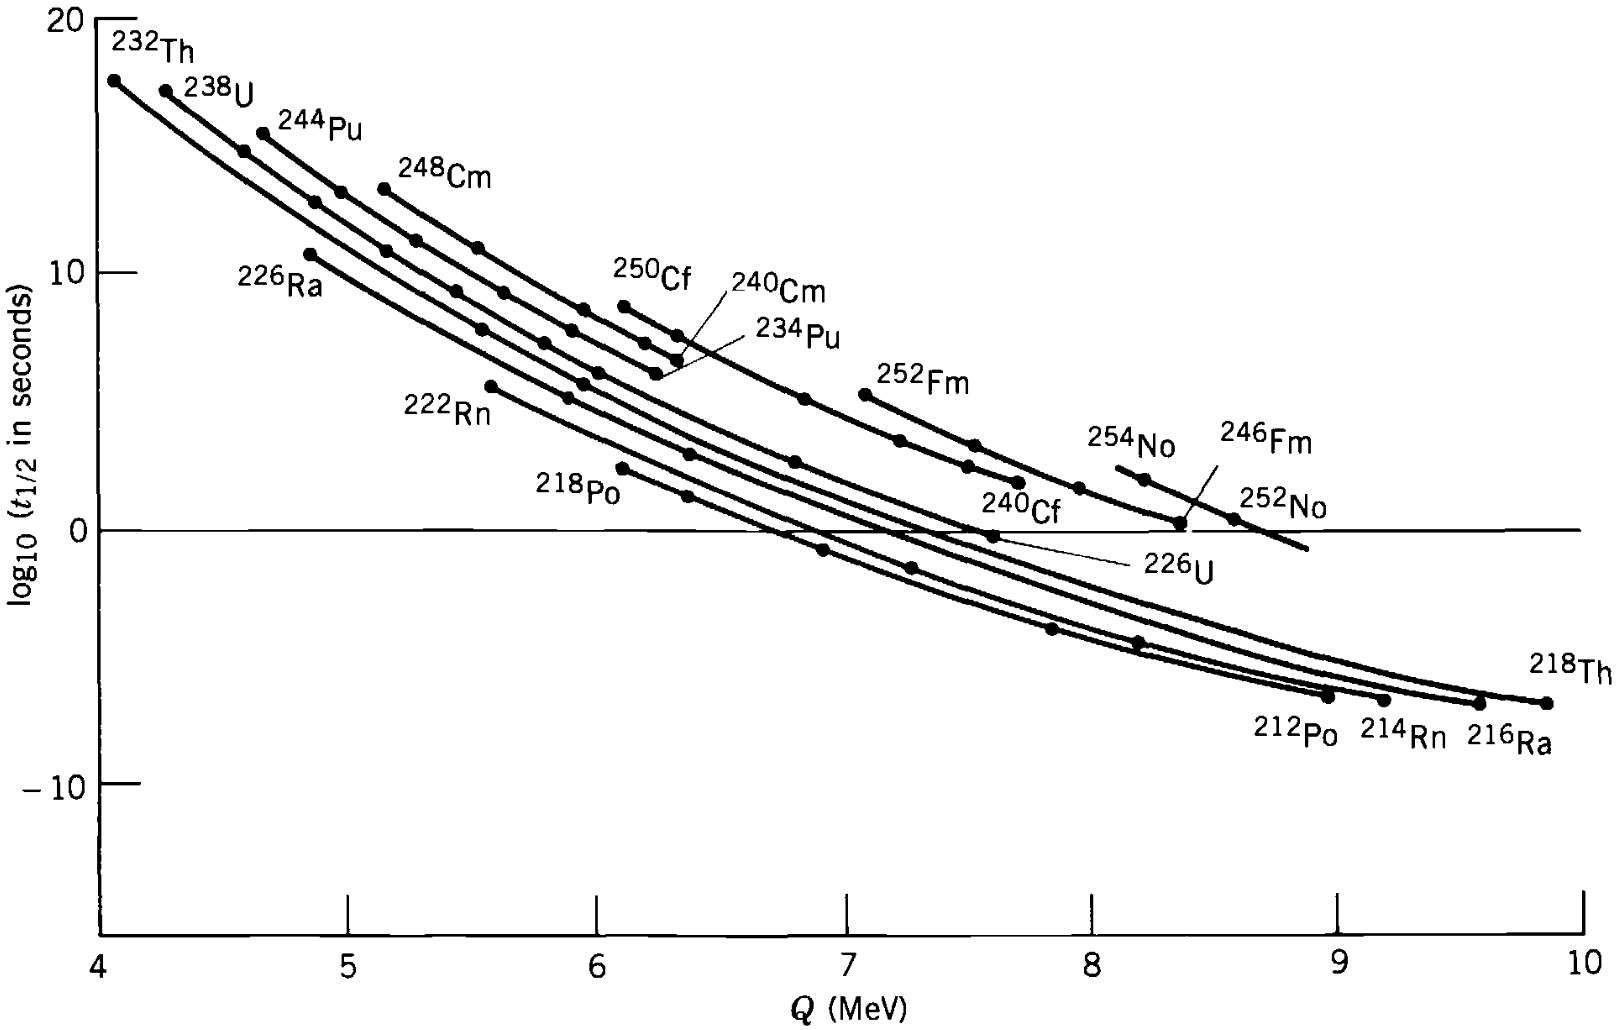
\includegraphics[width=0.75\textwidth]{geiger-nuttall.png}
	\caption{Legge di Geiger-Nuttal in famiglie isotopiche con nuclidi pari-pari.}
	\label{geiger-nuttall}
\end{figure}
\begin{figure}
	\centering
	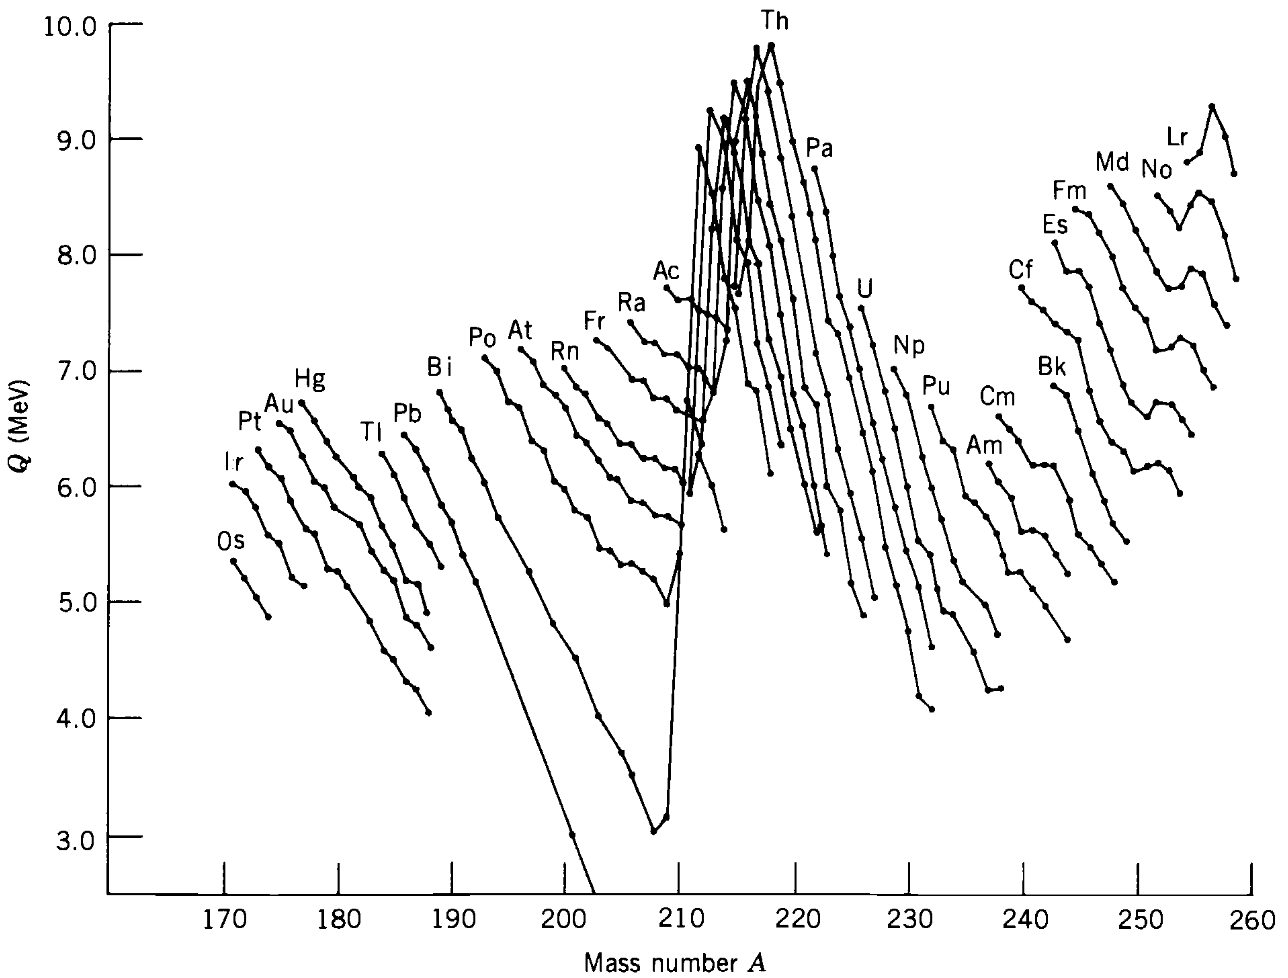
\includegraphics[width=0.75\textwidth]{gn-mass.png}
	\caption{Energia emessa per decadimento $ \alpha $ in famiglie isotopiche.}
	\label{gn-mass}
\end{figure}

\subsection{Teoria di Gamow}
\label{sec-gamow}

La prima interpretazione teorica del decadimento $ \alpha $ fu data da Gamow nel 1929, qualche anno dopo le osservazioni di Geiger e Nuttall.\\
È possibile pensare alla particella $ \alpha $ come un corpo stabile preformato all'interno del nuclide $ \ch{^A X} $ che periodicamente si viene a trovare sulla superficie del nucleo, ad una distanza $ R \equiv R_{\ch{Y}} + R_{\alpha} $. Il moto della particella $ \alpha $ è determinato dal'energia potenziale d'interazione col nucleo, plottata in Fig. \ref{alpha-pot}, che fu proposta da Gamow essere:
\begin{equation}
	U(r) =
	\begin{cases}
		-V_0 & r < R \\
		\frac{2(Z-2)e^2}{4\pi \epsilon_0 r} & r > R
	\end{cases}
	\label{eq:2.12}
\end{equation}
Il senso fisico di tale espressione è che in prossimità del nucleo a prevalere è la forza nucleare, che ha natura attrattiva, mentre allontanandosi da esso prevale l'interazione coulombiana, che è repulsiva: si vede quindi la presenza di una barriera coulombiana in $ r = R $.\\
Con una trattazione classica la particella $ \alpha $ sarebbe emessa solo se $ E_{\alpha} > U(R) $ e ciò avverrebbe in un tempo comparabile al tempo di attraversamento del nucleo, ovvero $ t \sim R / v_{\alpha} = R \sqrt{2E_{\alpha} / m_{\alpha}} $: stimando $ R \approx 1.2\fm \left( (A - 4)^{1/3} + 4^{1/3} \right) $, per un nucleo con $ A \sim 230 $ e $ Q \sim 4\mev $ si trova $ R \sim 9\fm $ e $ t \sim 10^{-21}\,\text{s} $, ovvero un decadimento praticamente istantaneo. Ciò però non è quello che si osserva sperimentalmente.\\
Quantisticamente, invece, grazie all'effetto tunnel è possibile che anche le particelle $ \alpha $ con $ E_{\alpha} < U(R) $ (cosa che è praticamente sempre, dato che $ U(R) \sim 20\mev $) possono essere emesse con probabilità inferiori e dunque tempi di decadimento più lunghi.\\
È possibile svolgere il calcolo esplicitamente approssimando il potenziale coulombiano tra $ r = R $ ed $ r = R_{\alpha} $ (determinato da $ U(R_{\alpha}) = E_{\alpha} $) come una successione di barriere di potenziale di spessore $ dr $: dalla meccanica quantistica è noto che un'onda (particella) incidente su una barriera di potenziale di spessore $ L $ risulta in un'onda riflessa e una trasmessa, le cui rispettive distribuzioni di probabilità (funzioni d'onda) sono determinate dai coefficienti di riflessione e trasmissione.

\begin{figure}[!hb]
	\centering
	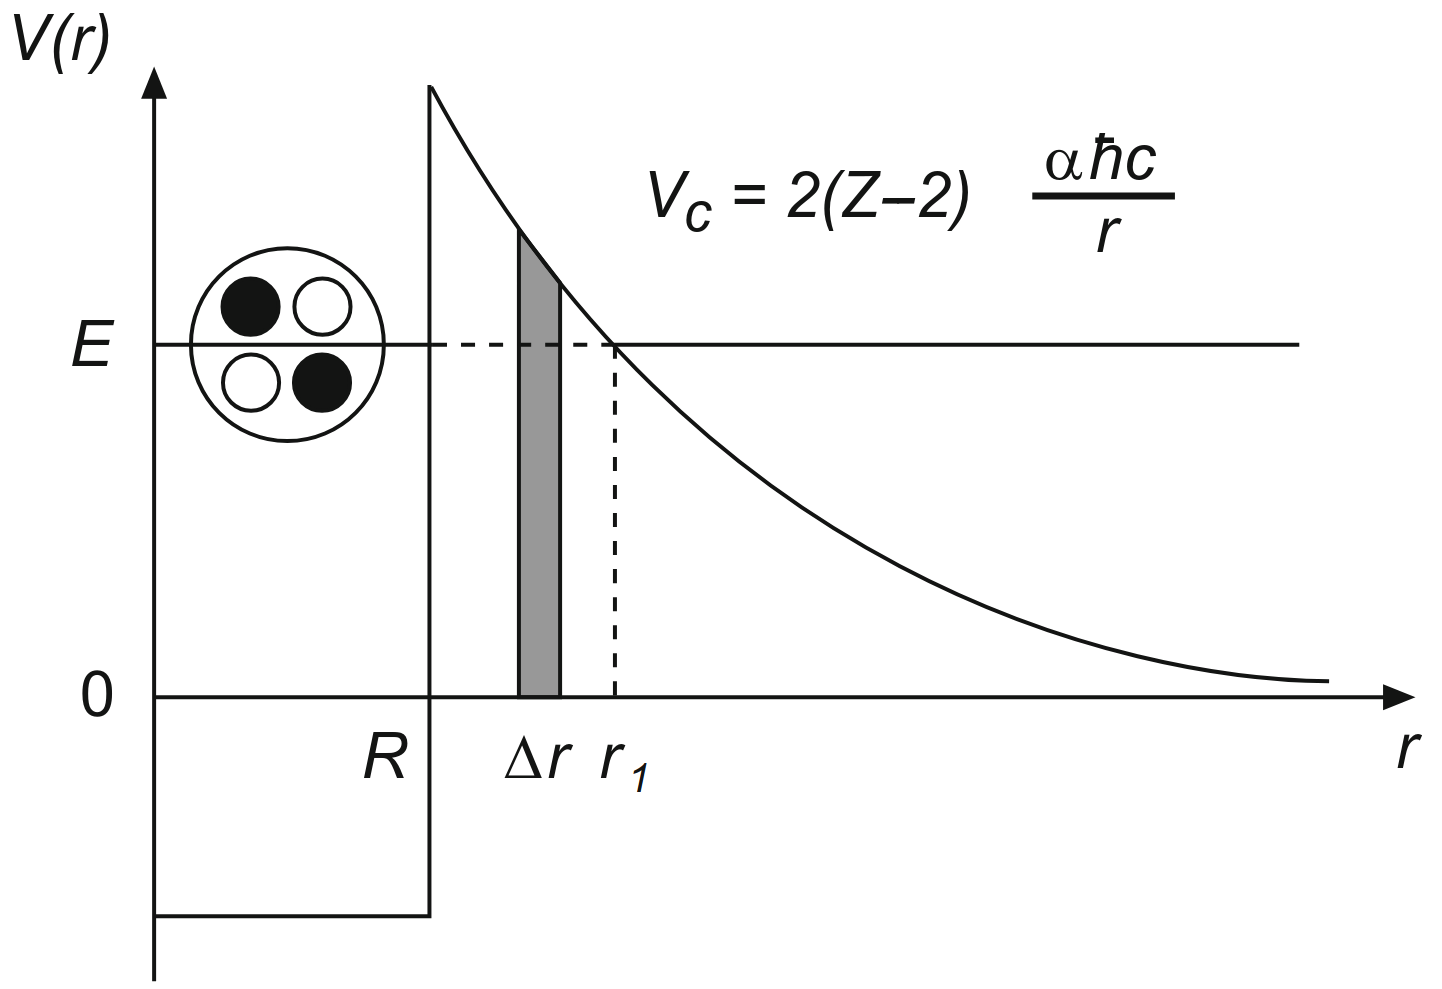
\includegraphics[width=0.60\textwidth]{alpha-pot.png}
	\caption{Potenziale d'interazione per il decadimento $ \alpha $.}
	\label{alpha-pot}
\end{figure}

Nel caso del decadimento $ \alpha $ è d'interesse solo il coefficiente di trasmissione nell'approssimazione $ E \ll V_0 $:
\begin{equation}
	T(E) = \left[ 1 + \frac{U_0^2}{4E (U_0 - E)} \sinh^2 \left( \frac{L}{\hbar} \sqrt { 2m (U_0 - E)} \right) \right]^{-1} \approx \frac{16 E (U_0 - E)}{U_0^2} e^{-2 \frac{L}{\hbar} \sqrt{2m (U_0 - E)}}
	\label{eq:2.13}
\end{equation}
Nel modello approssimato della successione di barriere di potenziale, quindi, si trova una probabilità di tunneling data da:
\begin{equation}
	P(E_{\alpha}) = \exp{\left[ -2 \int_{R}^{R_{\alpha}} dr \frac{1}{\hbar} \sqrt{2 m (U(r) - E_{\alpha}}) \right]} \eqdef e^{-2G}
	\label{eq:2.14}
\end{equation}
dove è stato definito il \textit{fattore di Gamow} $ G $. Svolgendo il calcolo col potenziale in Eq. \ref{eq:2.12} ed approssimando per una thick barrier $ R_{\alpha} \gg R $ (equivalente a $ E_{\alpha} \ll U(R) $, dato che dalla definizione $ R / R_{\alpha} = E_{\alpha} / U(R) $):
\begin{equation}
	\begin{split}
		G(E_{\alpha})
		&= \frac{2 (Z - 2) e^2}{\hbar} \sqrt{\frac{2m_{\alpha}}{E_\alpha}} \left[ \arccos \sqrt{\frac{R}{R_{\alpha}}} - \sqrt{\frac{R}{R_{\alpha}} - \frac{R^2}{R^2_{\alpha}}} \right]\\
		&\approx \frac{2 (Z - 2) e^2}{\hbar} \sqrt{\frac{2m_{\alpha}}{E_{\alpha}}} \left( \frac{\pi}{2} - \sqrt{\frac{R}{R_{\alpha}}} \right)
	\end{split}
	\label{eq:2.15}
\end{equation}
Questa espression mostra bene la fortissima dipendenza della probabilità di decadimento dall'energia della particella $ \alpha $: una piccola variazione di $ E_{\alpha} $ può portare $ P(E_{\alpha}) $ a variare di vari ordini di grandezza.\\
È anche possibile ricavare la legge di Geiger-Nuttall, dato che fenomenologicamente di può scrivere:
\begin{equation}
	\lambda = S \nu P(E_{\alpha})
	\label{eq:2.16}
\end{equation}
dove $ \lambda $ è la costante di decadimento, $ S $ è la probabilità che si formi una particella $ \alpha $ nel nucleo (può essere presa $ S \approx 1 $) e $ \nu $ è la knocking frequency, ovvero la frequenza con cui la particella $ \alpha $ urta con la barriera coulombiana. Si può stimare $ \nu $ a partire dal tempo che impiega la particella $ \alpha $ ad attraversare il nucleo (già trovato in precedenza): $ \nu \sim t^{-1} \sim 10^{21} \,\text{Hz} $. Dall'Eq. \ref{eq:2.16} si ha:
\begin{equation}
	\ln \lambda = \ln S + \ln \nu - 2 G(E_{\alpha}) \sim a(Z) - \frac{b(Z)}{\sqrt{E_{\alpha}}}
	\label{eq:2.17}
\end{equation}
che, ricordando che $ t_{1/2} = \frac{\ln 2}{\lambda} $, è proprio la legge di Geiger-Nuttall.\\
Ovviamente tutte queste relazioni sono qualitative e non quantitative, dato che sono state fatte alcune approssimazioni dalle quali la realtà si discosta notevolmente, prima su tutti la simmetria sferica: i nuclidi pesanti hanno forme notevolmente deformate (tendenti ad ellissoidi di rotazione), dunque le loro emissioni presentano notevoli anisotropie nella distribuzione angolare di particelle $ \alpha $.

\subsection{Spettri}

Per molti nuclidi che decadono tramite decadimento $ \alpha $ è possibile la presenza di più branch di decadimento, con percentuali di decadimento basse rispetto a quella dominante, che non portano direttamente allo stato fondamentale del nucleo figlio, ma a qualche suo stato eccitato: ciascuna di queste branch ha una propria energia di decadimento (deve essere sempre mono-energetico), e solitamente la branch con l'energia più alta è quella che va a popolare lo stato fondamentale del nucleo figlio.\\
Lo studio degli spettri di decadimento così prodotti (ad esempio immettendo le particelle $ \alpha $ in uno spettrometro magnetico) è importante per studiare i vari livelli energetici del nucleo figlio, specialmente nel caso in cui esso appartenga ad una specie nucleare di difficile sintesi.

\subsection{Cluster decay}

Spesso, quando un nuclide risulta instabile rispetto al decadimento per $ \ch{^4 He} $, esso lo è anche rispetto a quello per $ \ch{^8_4 Be} $, $ \ch{^{12}_6 C} $ ed altri nuclei, tendenzialmente formati da più particelle $ \alpha $, i cosiddetti \textit{nuclear clusters}. Anche questi sono sistemi particolarmente stabili preformati nel nucleo e, per un nuclear cluster di $ n $ particelle $ \alpha $, si può approssimare $ Q_n \sim Q_{\alpha}^n $: di conseguenza, per la legge di Geiger-Nuttall, i tempi di decadimento sono enormemente più lunghi rispetto a quelli del decadimento $ \alpha $, con conseguenza che i branching ratios sono praticamente trascurabili, sebbene occasionalmente questi cluster decays vengano osservati e siano stati ampiamente studiati.

\section{Fissione}

Dopo la scoperta del neutrone da parte di Chadwick nel 1932, furono condotti numerosi esperimenti nei quali vari nuclidi venivano irraggiati con neutroni: in particolare, Fermi et al. studiarono la radioattività a seguito della neutron capture, ottenendo il Nobel nel 1938 per gli studi sul decadimento $ \beta^- $, mentre Meitner e Hahn osservarono la fissione negli elementi transuranici.

\paragraph{Neutroni}

Si utilizza una specifica terminologia per classificare i neutroni in base alla loro energia $ E_n $:
\begin{enumerate}
	\item high energy neutrons: $ E_n > 100\mev $;
	\item fast neutrons: $ 100\kev < E_n < 100\mev $;
	\item epithermal neutrons: $ 0.1\ev < E_n < 100\kev $;
	\item thermal/slow neutrons: $ 1\,\text{meV} < E_n < 0.1\ev $,
	\item cold/ultracold neutrons: $ E_n < 1\,\text{meV} $.
\end{enumerate}
Come si può vedere in Fig. \ref{fission-cs}, sperimentalmente si trova che i neutroni a basse energie, specialmente i thermal neutrons, sono quelli più efficaci per indurre reazioni di fissione nucleare.

\begin{figure}
	\centering
	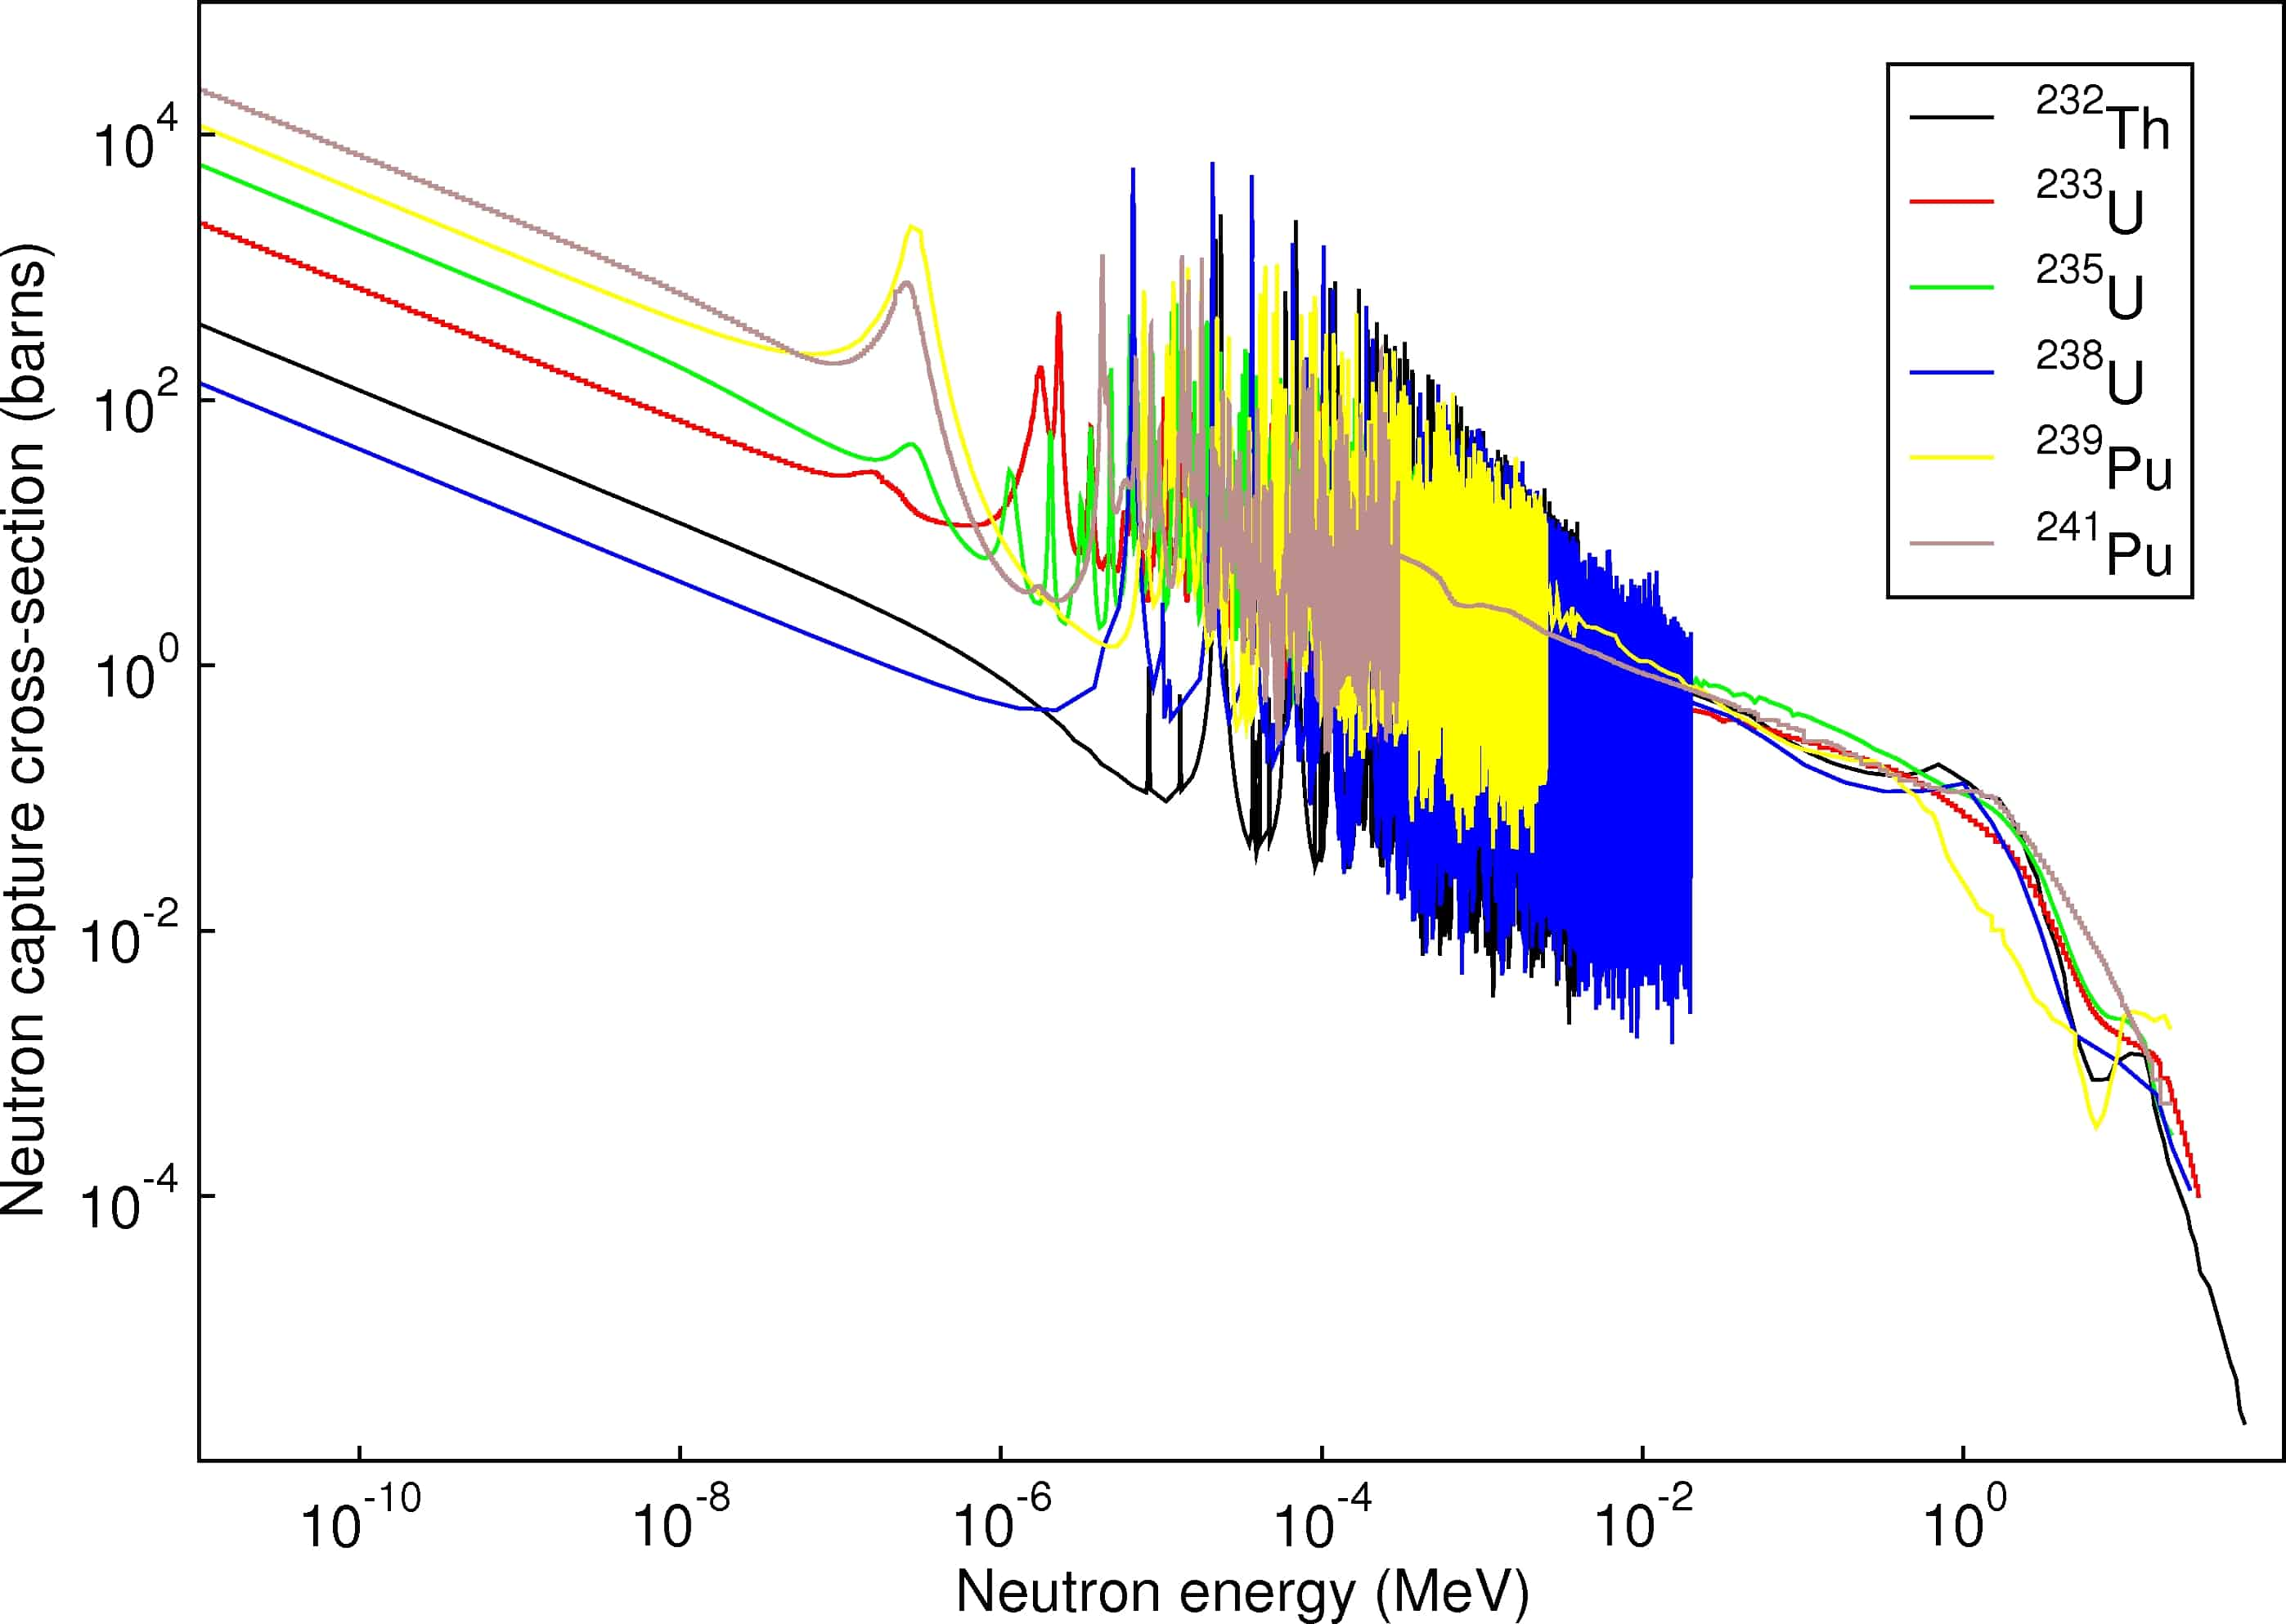
\includegraphics[width=0.75\textwidth]{fission-cs.jpg}
	\caption{Neutron-induced fission cross-section.}
	\label{fission-cs}
\end{figure}
\begin{figure}
	\centering
	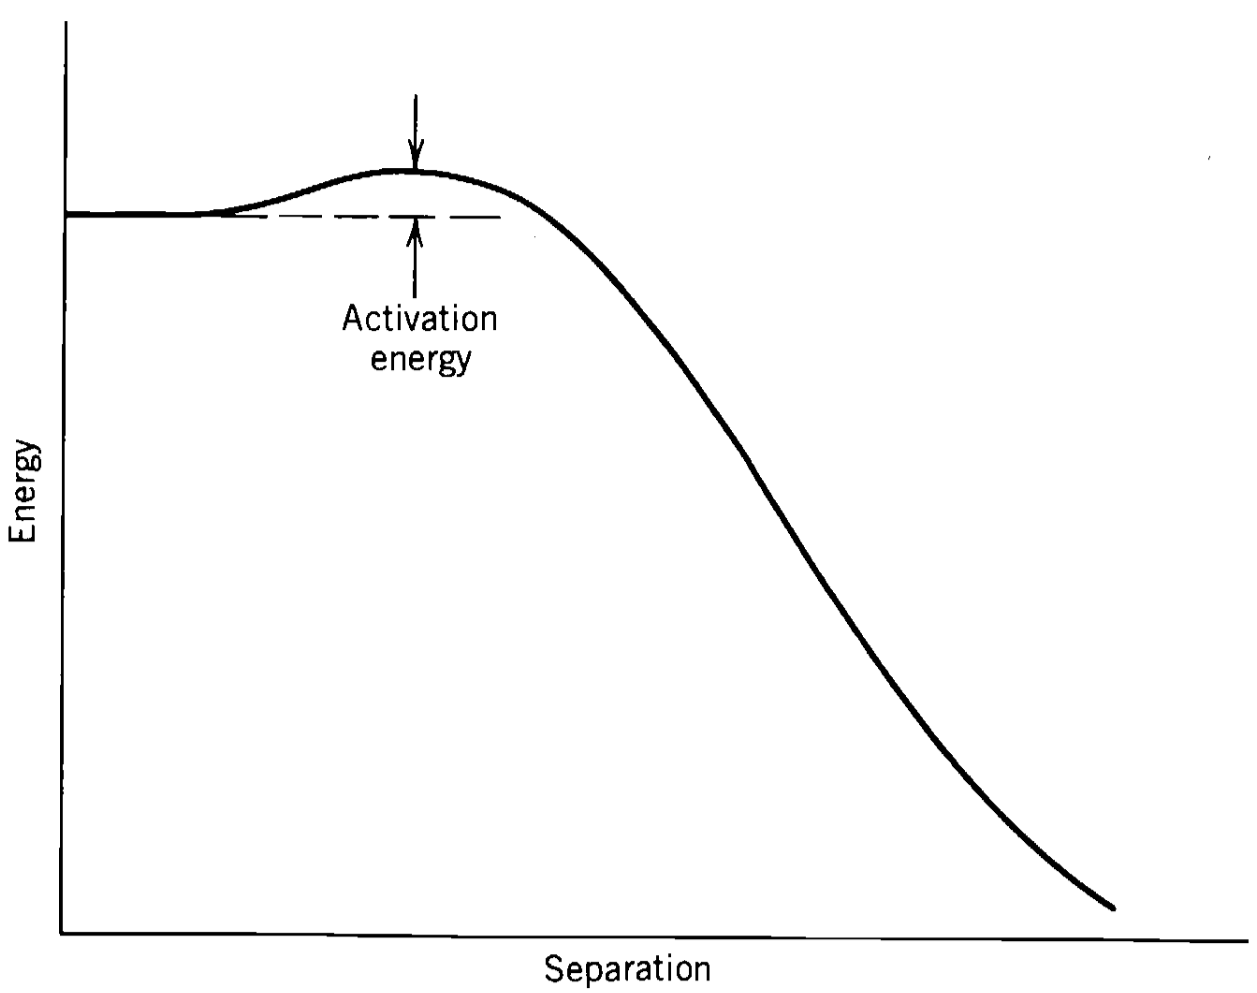
\includegraphics[width=0.75\textwidth]{fission-pot.png}
	\caption{Coulomb potential in a fissioning nucleus.}
	\label{fission-pot}
\end{figure}

\subsection{Fissione spontanea}

La tendenza dei nuclei pesanti a fissionare è evidente dall'andamento della binding energy rispetto ad $ A $ (Fig. \ref{bind-en}): ad esempio, se si considera la fissione dell'uranio $ \ch{^{235}_{92} U} \rightarrow \ch{^{90}_{36} Kr} + \ch{^{142}_{56} Ba} + 3 n $, il $ Q $-value della reazione è $ 166.73\mev $, dunque è una reazione energeticamente fortemente favorita. Va però notato che il decay branch per decadimento $ \alpha $ è fortemente dominante in natura, basta confrontare, ad esempio, i seguenti decadimenti:
\begin{equation*}
	\begin{split}
		\ch{^{238}_{92} U} \xrightarrow{4\,\text{Gy}} \ch{^{234}_{90} Th} + \alpha &\qquad \ch{^{238}_{92} U} \xrightarrow{\sim 10^7\,\text{Gy}} \ch{^{140}_{54} Xe} + \ch{^{96}_{38} Sr} + 2n\\
		\ch{^{235}_{92} U} \xrightarrow{0.7\,\text{Gy}} \ch{^{231}_{90} Th} + \alpha &\qquad \ch{^{235}_{92} U} \xrightarrow{\sim 10^8\,\text{Gy}} \ch{^{142}_{56} Ba} + \ch{^{90}_{36} Kr} + 3n
	\end{split}
\end{equation*}
La fissione è osservata solo in nuclei pesanti (il nuclide fissile più leggero è $ \ch{^{226}_{88} Ra} $), e la fissione spontanea diventa il decay mode dominante solo in nuclidi con $ A \ge 250 $.\\
Ciò che inibisce la fissione è una barriera coulombiana analoga a quella del decadimento $ \alpha $: in questo caso, però, essa ha un andamento liscio (in senso analitico), com'è possibile vedere in Fig. \ref{fission-pot}. L'energia necessaria affinché i due prodotti della fissione (supposti preformati) oltrepassino la barriera coulombiana è, nella maggior parte dei casi, troppo alta per rendere la fissione un decay mode significativo; a livello teorico, dovrebbero esistere anche dei nuclidi in cui la barriera si annulla, ovvero in cui i due prodotti hanno sempre l'energia necessaria per superarla, e tali nuclidi dovrebbero fissionare istantaneamente: naturalmente essi non esistono in natura, e si dovrebbero trovare attorno ad $ A = 300 $.\\
L'altezza della barriera coulombiana rispetto all'energia del ground state è detta activation energy ed è possibile calcolarla sia assumendo il modello semplificato a goccia sia tenendo conto degli effetti delle shell nucleari: entrambi i casi sono plottati in Fig. \ref{act-en}.

\begin{figure}
	\centering
	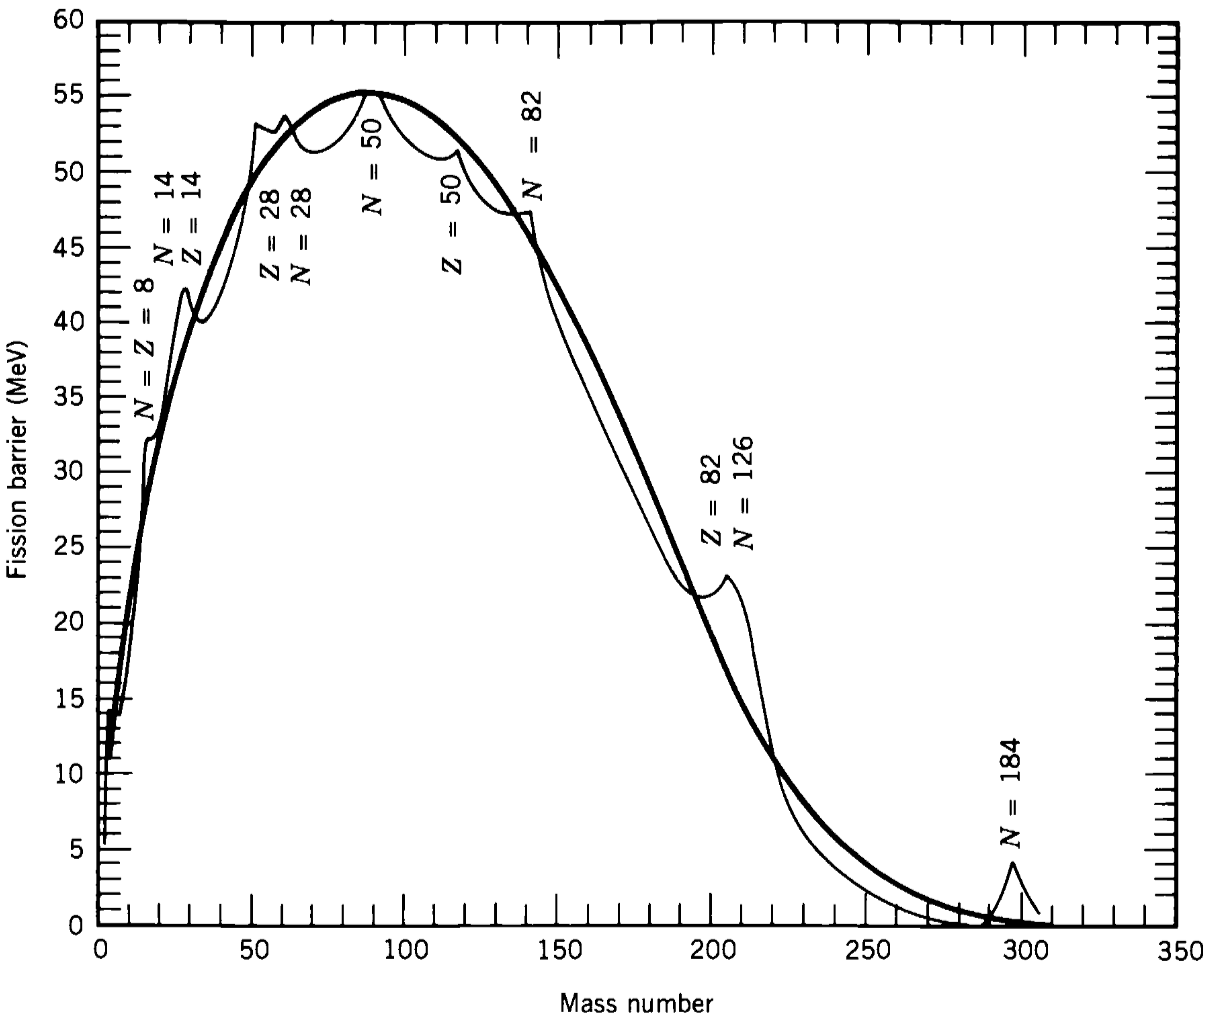
\includegraphics[width=0.65\textwidth]{act-en.png}
	\caption{Activation energy of nuclear fission.}
	\label{act-en}
\end{figure}
\begin{figure}
	\centering
	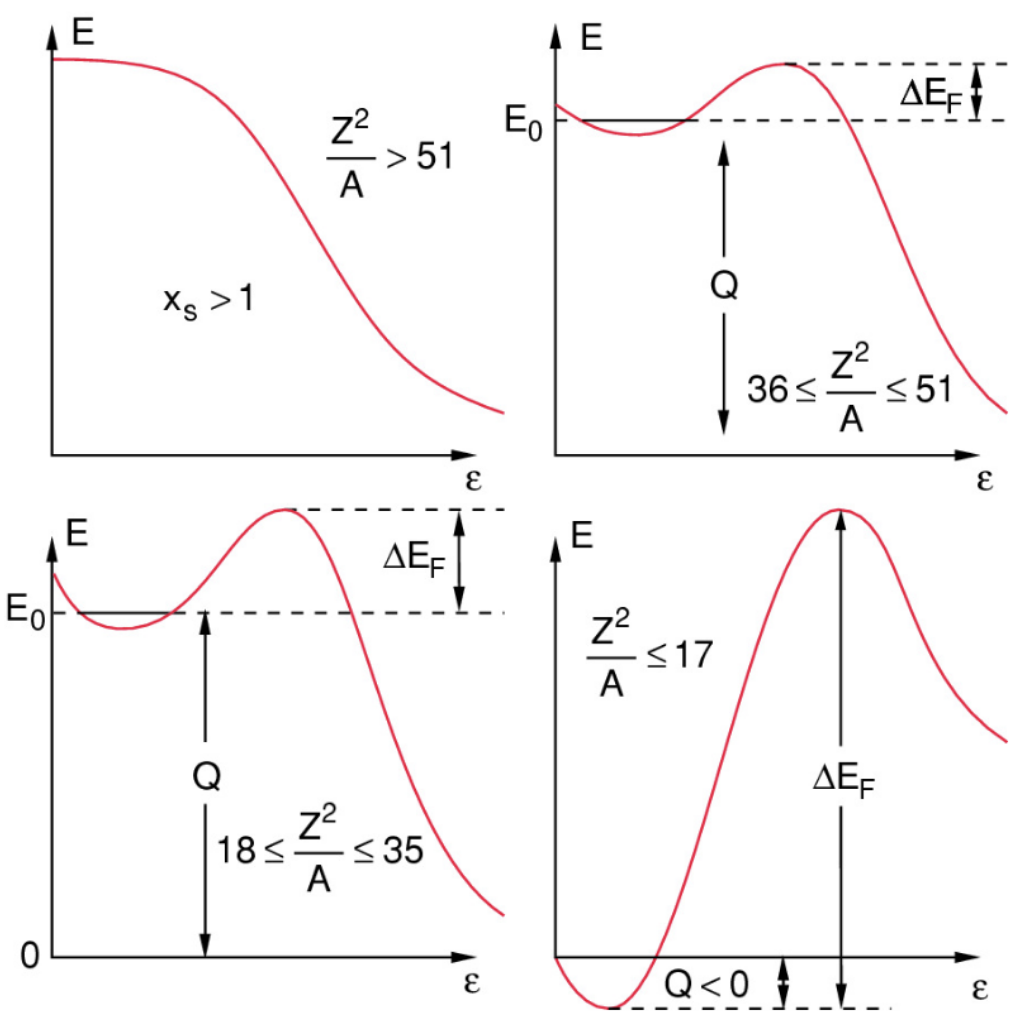
\includegraphics[width=0.60\textwidth]{act-en-z.png}
	\caption{Potential barrier as a funzion of the deformation parameter for various fissility values.}
	\label{act-en-z}
\end{figure}

\paragraph{Liquid drop model}

Semplificando, questo modello considera solo le proprietà nucleari medie, assumendo un nuclide sferico nel suo ground state. Nel caso di un nucleo fissile, l'instabilità porta ad una deformazione del nuclide in un ellissoide: assumendo il raggio iniziale $ R $ e l'eccentricità dell'ellissoide $ \varepsilon $, si possono calcolare i semiassi come:
\begin{equation}
	a = R \left( 1 + \varepsilon \right) \qquad b = R \left( 1 + \varepsilon \right)^{-1/2}
	\label{eq:2.18}
\end{equation}
Si vede dunque che il volume $ V = \frac{4}{3}\pi R^3 = \frac{4}{3} \pi ab^2 $ rimane inalterato, mentre la superficie varia di un fattore approssimabile ad $ \varepsilon $: $ S = 4\pi R^2 \left( 1 + \frac{2}{5} \varepsilon^2 + \dots \right) $; analogamente, si mostra che l'energia d'interazione coulombiana varia di un fattore $ \left( 1 - \frac{1}{5} \varepsilon^2 + \dots \right) $.\\
Dalla formula semi-empirica di Weizsäcker (Eq. \ref{eq:1.30}) deriva che, a seguito della deformazione, la binding energy varia di:
\begin{equation}
	\Delta B = - a_S A^{2/3} \left( 1 + \frac{2}{5} \varepsilon^2 + \dots \right) - a_C \frac{Z^2}{A^{1/3}} \left( 1 - \frac{1}{5} \varepsilon^2 + \dots \right) \approx \left( -\frac{2}{5} a_S A^{2/3} + \frac{1}{5} a_C \frac{Z^2}{A^{1/3}} \right) \varepsilon^2
	\label{eq:2.19}
\end{equation}
Se $ \Delta B > 0 $, il nucleo risulta instabile rispetto alla deformazione e fissiona, dunque si trova una condizione per la fissione spontanea:
\begin{equation}
	\Chi \defeq \frac{a_C}{2a_S} \frac{Z^2}{A} > 1
	\label{eq:2.20}
\end{equation}
dove è stata definita la fissility $ \Chi $. Utilizzando i valori di $ a_S $ ed $ a_C $ interpolati si trova la condizione $ Z^2 / A > 51 $, ovvero $ Z > 114 $ e $ A > 270 $; al di sotto di questi valori la fissione è possibile solo fornendo la necessaria energia di attivazione (vedere Fig. \ref{act-en-z}).\\
Bisogna specificare che per $ Z^2 / A > 51 $ la fissione spontanea è istantanea, mentre per nuclidi con $ Z^2 / A \lesssim 51 $ è possibile anche una delayed fission per effetto tunnel (a causa della repulsione tra protoni), analogamente al decadimento $ \alpha $, ma nella maggior parte dei casi quest'ultimo è dominante.
Infine, si può notare in Fig. \ref{fission-lt} come i tempi di decadimento aumentino al diminuire di $ Z^2 / A $.

\begin{figure}[!hb]
	\centering
	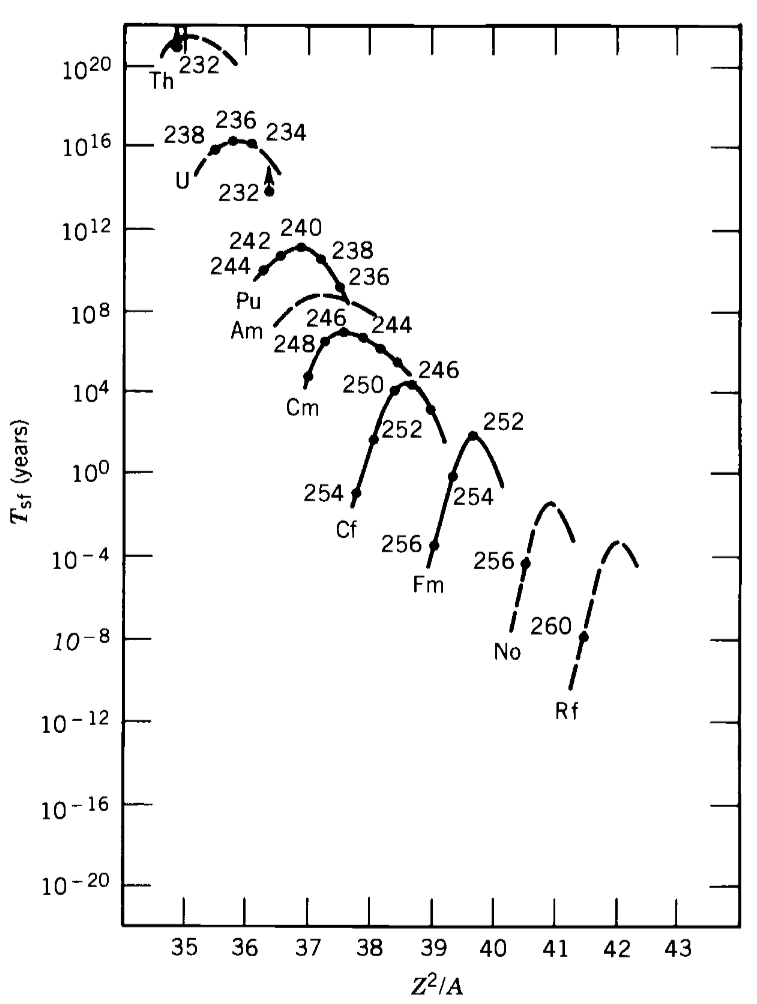
\includegraphics[width=0.80\textwidth]{fission-lt.png}
	\caption{Lifetimes for spontaneous fission.}
	\label{fission-lt}
\end{figure}

\subsection{Fissione indotta}

Dato che i neutroni non sono affetti dal potenziale coulombiano, è possibile indurre la fissione di un nuclide facendolo scatterare con un neutrone termico. Bisogna però notare una differenza tra la fissione di nuclidi pari-pari e nuclidi pari-dispari, dovuta al termine di pairing nella formula di Weizsäcker (Eq. \ref{eq:1.30}).\\
Si considerino ad esempio due campioni di $ \ch{^{235}_{92} U} $ e $ \ch{^{238}_{92} U} $ e li si irraggi con neutroni termici:
\begin{enumerate}
	\item $ \ch{^{235}_{92} U} + n \rightarrow \ch{^{236}_{92} U}^* $: $ Q = 6.5\mev > \Delta E_F = 6.1\mev $;
	\item $ \ch{^{238}_{92} U} + n \rightarrow \ch{^{239}_{92} U}^* $: $ Q = 4.8\mev < \Delta E_F = 6.4\mev $;
\end{enumerate}
Si vede dunque che la fissione di $ \ch{^{235}_{92} U} $ può avvenire con neutroni termici, mentre per quella di $ \ch{^{238}_{92} U} $ sono necessari neutroni veloci. Ciò è dovuto al fatto che i nuclidi pari-pari sono energeticamente favoriti, dunque il termine di pairing favorisce processi da pari-dispari a pari-pari, mentre ostacola quelli da pari-pari a pari-dispari: nel caso considerato, infatti, la differenza di energia ammonta a $ \Delta E = \delta (236^{-1/2} + 238^{-1/2}) = 1.5\mev $.\\
È interessante notare che $ \ch{^{235}_{92} U} $ e $ \ch{^{238}_{92} U} $ sono gli unici isotopi dell'uranio rimasti in natura, con abbondanze isotopiche rispettivamente del $ 0.72\% $ e $ 99.28\% $ e sezioni d'urto $\sigma(235) = 589 \, \text{barn} \, (E_\text{n}=0.025 \, \text{eV})$ e $\sigma(238) = 0.5 \, \text{barn} \, (E_\text{n}>1.8 \, \text{MeV})$.

\subsection{Caratteristiche}

Il processo di fissione del nuclide non presenta grosse differenze tra il caso spontaneo e quello indotto: in maniera quasi istantanea ($ \sim 10^{-17}\,\text{s} $) il nucleo si deforma radicalmente andando a formare i due frammenti di fissione (sono possibili fissioni ternarie ma sono estremamente rare), i quali si separano in tempi brevissimi ($ \sim 10^{-14}\,\text{s} $): questi sono nuclidi molto neutron-rich, dunque espellono i neutroni con energie di legame superiori all'energia di legame media, andando così a formare i prodotti di fissione; quest'ultimi possono decadere tramite decadimenti $ \beta $ e $ \gamma $, con tempi su una scala dai secondi ai milioni di anni, muovendosi verso la valle di stabilità.

\subsubsection{Asimmetria di fissione}

I due frammenti altamente eccitati in cui si separa il nucleo a seguito della fissione non sono uguali, ma presentano una notevole asimmetria; per di più, variando il nuclide fissile si osserva che la distribuzione dei frammenti pesanti rimane praticamente inalterata, mentre la massa in eccesso viene inglobata dai frammenti leggeri (vedere Fig. \ref{fission-md}).\\
Ciò può essere spiegato dal fatto che la fissione, sebbene trattata in maniera elementare utilizzando il liquid drop model, risente in realtà degli effetti delle shell nucleari: come si può notare in Fig. \ref{fission-asimm}, la distribuzione dei frammenti pesanti si sovrappone ad una regione di completamento di shell nucleari, con la presenza anche del nuclide doubly-magic $ \ch{^{132}_{50} Sn_{82}} $, che ha una configurazione estremamente stabile; tutto ciò non accade, invece, per la distribuzione dei frammenti leggeri, i quali non si sovrappongono a nessun magic nucleus.\\
Circa metà dei prodotti di fissione decadono in meno di un anno, mentre i restanti possono avere tempi di decadimento anche di milioni di anni: questi formano le scorie radioattive.\\
I prodotti di fissione sono molto neutron-rich, dunque per la maggior parte sono instabili per decadimento $ \beta^- $: la fissione nucleare è un importante strumento di ricerca per la regione $ \beta^- $-instabile, difficilmente raggiungibile con altri metodi: i prodotti di fissione possono dar luogo ad intere catene di decadimenti $ \beta^- $.

\begin{figure}
	\centering
	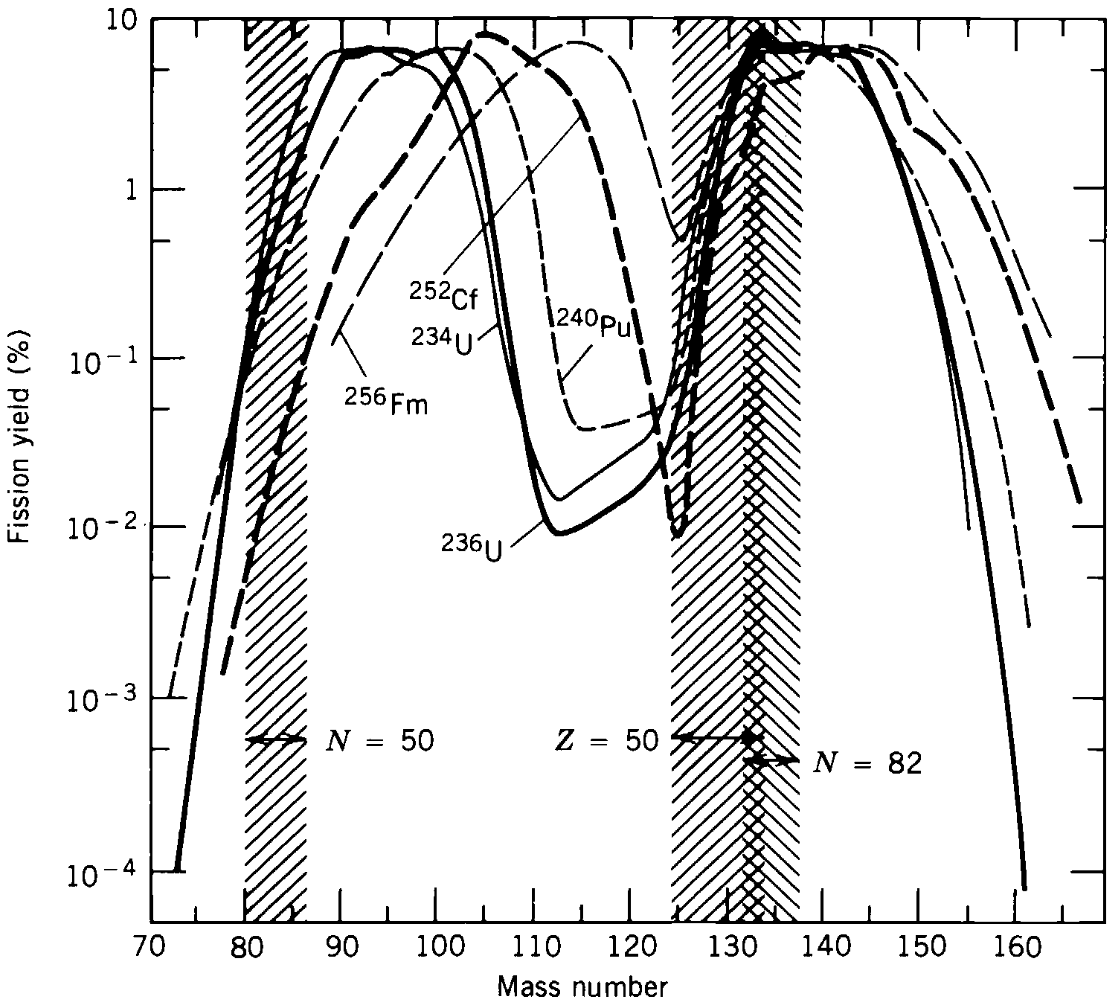
\includegraphics[width=0.60\textwidth]{fission-asimm.png}
	\caption{Asimmetry in fission products.}
	\label{fission-asimm}
\end{figure}
\begin{figure}
	\centering
	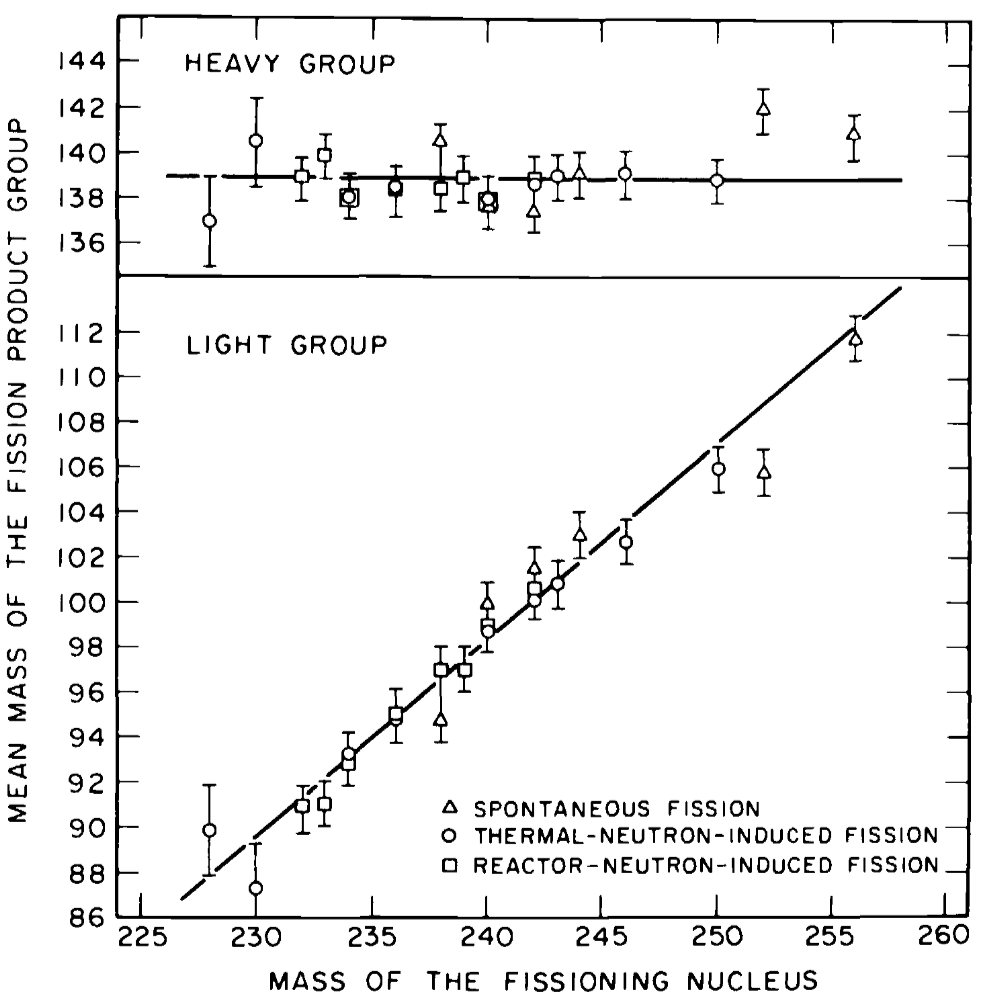
\includegraphics[width=0.60\textwidth]{fission-md.png}
	\caption{Distributions of light and heavy fission products.}
	\label{fission-md}
\end{figure}

\subsubsection{Emissione di neutroni}

I neutroni prodotti dalla fissione di un nuclide si possono distinguere in due categorie: prompt neutrons and delayed neutrons.\\
I prompt neutrons vengono emessi praticamente in contemporanea al processo di fissione, venendo emessi dal nuclide fissile e dai frammenti di fissione: il numero di prompt neutrons viene indicato come $ \nu_n $ e generalmente si ha $ \langle \nu_n \rangle \approx 2.4 $.\\
La distribuzione di prompt neutrons in base alla loro energia cinetica è una distribuzione di Maxwell, mentre $ \nu_n $ si distribuisce secondo una gaussiana indipendentemente dalla fissione considerata, come visibile in Fig. \ref{n-neut-dist}: i prompt neutrons vengono prodotti con energia di circa $ 2\mev $, in media.\\
I delayed neutrons, d'altro canto, sono quelli prodotti nelle decay chains iniziate dai prodotti di fissione, solitamente tra $ 0.2\,\text{s} $ e $ 60\,\text{s} $ dopo la fissione, e costituiscono appena l'$ 1\% $ dei neutroni totali prodotti dalla fissione.

\begin{figure}[!b]
	\centering
	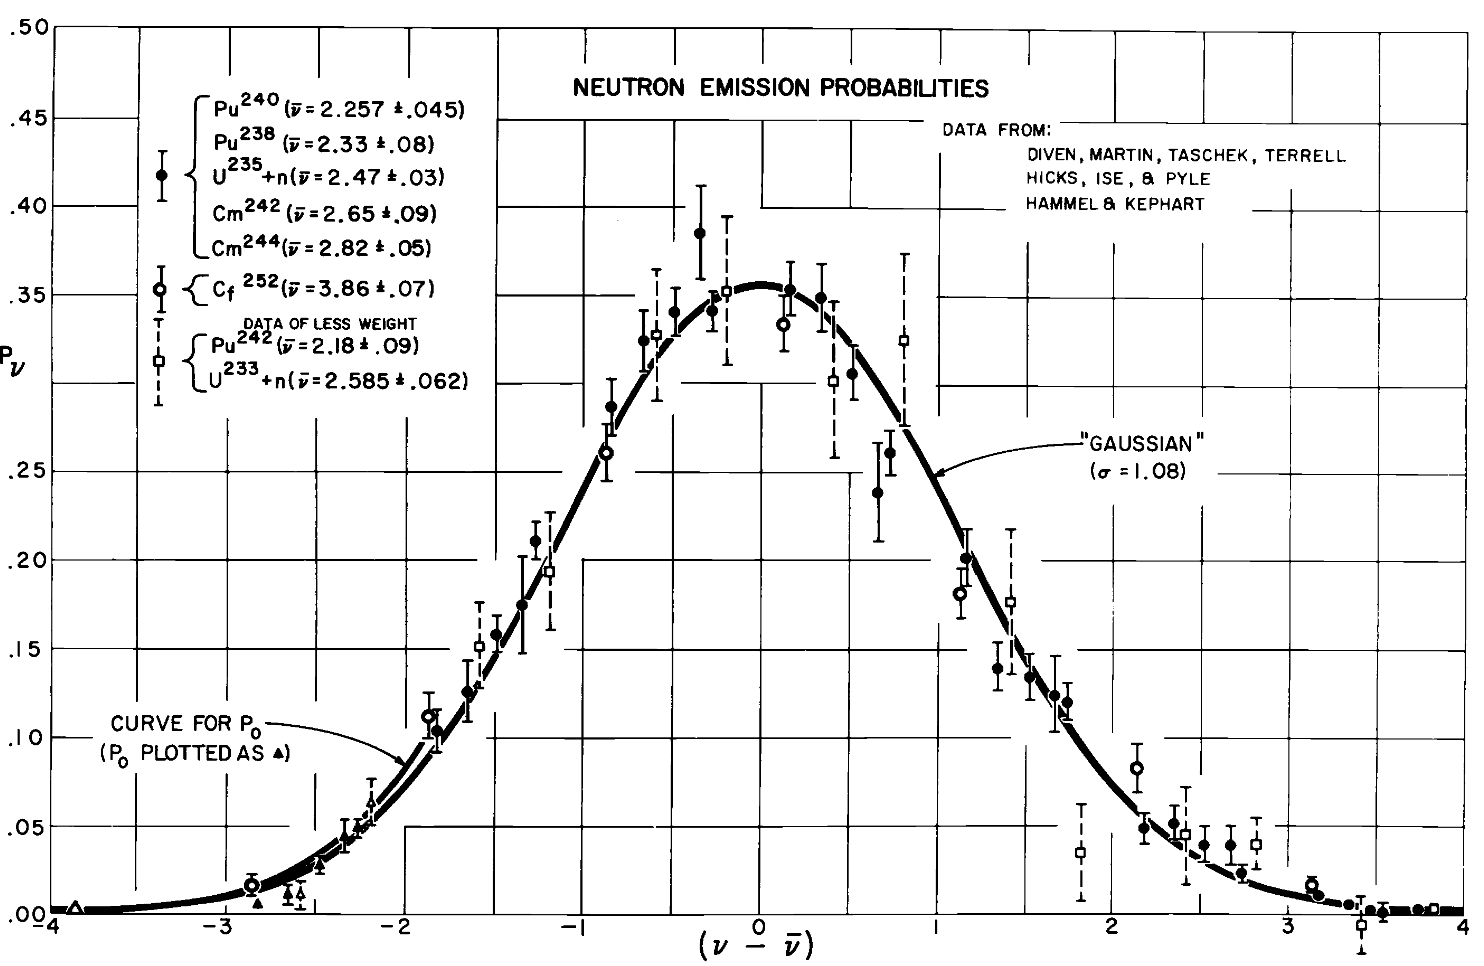
\includegraphics[width=0.75\textwidth]{n-neut-d.png}
	\caption{Prompt neutrons' number distribution.}
	\label{n-neut-dist}
\end{figure}

\subsubsection{Bilancio energetico}

Considerando, ad esempio, la fissione del $ \ch{^{235}_{92} U} $, i $ 210\mev $ di energia rilasciata vengono ripartiti nel seguente modo:
\begin{enumerate}
	\item frammenti di reazione: $ \ch{Y}_{\text{small}} \approx 100\mev $ e $ \ch{Y}_{\text{large}} \approx 70\mev $;
	\item prompt emissions: neutrons $ \approx 5\mev $ e fotoni $ \approx 7\mev $;
	\item decadimenti: $ \beta^- \approx 20\mev $ (di cui $ \approx 12\mev $ persi in neutrini) e $ \gamma \approx 8\mev $.
\end{enumerate}
La differenza tra i due frammenti è dovuta alla conservazione del momento lineare: trascurando i neutroni si ha $ m_1 \ve{v}_1 = m_2 \ve{v}_2 $, dunque $ K_1 / K_2 = m_2 / m_1 $, ovvero il frammento leggero acquista la maggior parte del'energia cinetica disponibile.

\subsection{Applicazioni}

\subsubsection{Studio della stuttura nucleare}

Dato che la fissione produce nuclidi neutron-rich eccitati molto esotici, essa può essere usata per studiare una zona difficilmente popolabile della nuclear chart, quella $ \beta^- $-instabile.\\
Inoltre, a partire dalla fissione è possibile ottenere la cosiddetta spallazione del nuclide fissile: quando l'energia della particella proiettile è molto elevata la fissione produce frammenti multipli. Essendo il processo non più binario, la distribuzione dei frammenti non è più a doppia campana (come in Fig. \ref{fission-asimm}), ma si va a popolare anche la conca centrale: più è alta l'energia del proiettile, più saranno i frammenti di masse intermedie prodotti.\\
Questo, ad esempio, è ciò che avviene nell'esperimento ISOLDE al CERN: nuclei esotici vengono prodotti con irraggiamento di protoni, i quali, provenendo da LHC, hanno energie dell'ordine di $ 1.5\gev $.

\subsubsection{Reattori a fissione}

Il funzionamento dei reattori a fissione nucleare si basa sulle reazioni a catena dell'uranio: queste avvengono poiché la fissione di $ \ch{^{235}_{92} U} $ produce in media 3 neutroni, i quali potenzialmente possono dar luogo ad ulteriori fissioni.\\
Il problema principale è che $ \ch{^{235}_{92} U} $ richiede un neutrone termico per fissionare, mentre i neutroni prodotti dalla fissione sono neutroni veloci: per rallentare questi neutroni, è necessario alternare nel reattore strati di materiale fissile a strati di materiale moderatore. Quest'ultimo solitamente è costituito da acqua o da grafite, materiali leggeri con una cross-section elevata per scattering neutronico (elastico) ai quali viene ceduta una grande frazione dell'energia cinetica.\\
È inoltre necessaria, come materiale fissile, una miscela di uranio con almeno il $ 3\% $ di $ \ch{^{235}_{92} U} $: per fare ciò, è necessario arricchire l'uranio estratto in natura. Il $ \ch{^{238}_{92} U} $ non è inerte, ma può fissionare quando dei neutroni veloci sfuggono alle barre di moderazione.\\
Per mantenere la reazione sotto controllo bisogna avere il giusto numero di neutroni: se non vengono prodotti abbastanza neutroni dalle fissioni la catena non riesce ad autosostenersi, mentre se ne vengono prodotti troppi c'è il rischio che essa non sia più controllabile ed esploda esponenzialmente. In particolare, data una certa massa di materiale fissile, si definisce il neutron reproduction factor $ k $ come il rapporto tra i numeri di neutroni fissili (quelli che effettivamente danno luogo a fissioni) di due generazioni successive di nuclidi fissili a catena avviata: la massa si dice critica se $ k = 1 $, supercritica se $ k > 1 $ e subcritica se $ k < 1 $.\\
L'obiettivo, in un reattore a fissione, è mantenere il materiale fissile in stato critico, dunque controllabile: per mantenere la catena sotto controllo si utilizzano delle barre fatte di materiale ad alto potere d'assorbimento di neutroni (ad esempio bario, boro, cadmio, indio etc.), le quali possono essere inserite all'interno del materiale fissile per bloccare totalmente o in parte la reazione.\\
Un altro parametro importante nella caratterizzazione di un reattore a fissione è il numero medio di neutroni termici fissili: infatti, non tutti i neutroni termici prodotti da fissione generano a loro volta delle fissioni, poiché subentrano processi d'assorbimento. Considerando del materiale fissile composto da $ \ch{X}_i $ specie nucleari con frazioni $ x_i $, si hanno le cross-section di fissione e di assorbimento
\begin{equation}
	\sigma_f = \sum_{i} x_i \sigma_f\left( \ch{X}_i \right) \qquad \sigma_a = \sum_{i} x_i \sigma_a\left( \ch{X}_i \right)
	\label{eq:2.21}
\end{equation}
Il numero medio di neutroni termici fissili $ \eta $ risulta essere dunque:
\begin{equation}
	\eta = \frac{\sigma_f}{\sigma_f + \sigma_a} \langle \nu_n \rangle
	\label{eq:2.22}
\end{equation}
Ad esempio, per una miscela naturale di $ \ch{^{235}_{92} U} $ al $ 0.72\% $ e $ \ch{^{238}_{92} U} $ al $ 99.28\% $, dato che $ \sigma_f(235) = 584\,\text{barn} $, $ \sigma_a(235) = 97\,\text{barn} $, $ \sigma_f(238) = 0 $ ($ \ch{^{238}_{92} U} $ non fissiona con neutroni termici) e $ \sigma_a(238) = 2.75\,\text{barn} $, si hanno $ \sigma_f = 4.20\,\text{barn} $ e $ \sigma_{a} = 3.43\,\text{barn} $, quindi $ \eta = 1.33 $.\\
Considerando invece una miscela con $ \ch{^{235}_{92} U} $ arricchito al $ 3\% $, si ottiene $ \eta = 1.84 $, che permette una maggior perdita neutronica per altri processi d'assorbimento senza entrare in regime subcritico.

\section{Decadimento \texorpdfstring{$ \beta $}{TEXT}}

Il termine \textit{decadimento $ \beta $} indica collettivamente tutte le transizioni tra isobari (stesso $ A $) mediate dall'interazione debole: questi processi tendono ad ottimizzare il rapporto $ N/Z $ dei nuclidi, percorrendo catene isobariche verso la valle di stabilità. In particolare, in questi decadimenti l'interazione debole cambia un neutrone in un protone (o viceversa), producendo una coppia leptone-antileptone o trasformando un elettrone in un neutrino.\\
Si distinguono tre decadimenti separati:
\begin{enumerate}
	\item decadimento $ \beta^- $: $ n \rightarrow p^+ + e^- + \bar{\nu}_e $;
	\item decadimento $ \beta^+ $: $ p^+ \rightarrow n + e^+ + \nu_e $;
	\item electron capture: $ p^+ + e^- \rightarrow n + \nu_e $.
\end{enumerate}
Nel caso dell'electron capture avviene che un elettrone delle shell più interne (tipicamente la shell K), il quale ha un alta probabilità di trovarsi all'interno del nucleo, venga catturato da quest'ultimo, lasciando un buco nella shell che viene subito colmato da una transizione a catena degli elettroni dell'atomo, emettendo dei raggi X caratteristici.

\subsection{Decadimento dei nucleoni}

Il decadimento $ \beta^+ $ del protone e quello $ \beta^- $ del neutrone possono essere spiegati tramite il modello a quark dei nucleoni.\\
Il protone è formato da due quark up ed un quark down: nel caso in cui esso sia parte di un nucleo può accadere che, tramite interazione debole, un quark up diventi un quark down, come mostrato nel seguente diagramma di Feynman:

\begin{figure}[h!]
	\centering
\begin{tikzpicture}
	\begin{feynman}
		\vertex (a1) {\(u\)};
		\vertex[right=4cm of a1] (ai);
		\vertex[right=4cm of ai] (a2) {\(d\)};

		\vertex[below=2em of a1] (b1) {\(u\)};
		\vertex[below=2em of b1] (c1) {\(d\)};
		\vertex[below=2em of a2] (b2) {\(u\)};
		\vertex[below=2em of b2] (c2) {\(d\)};

		\vertex[above=1.5cm of a2] (d1) {\(\nu_e\)};
		\vertex[above=3em of d1] (d2) {\(e^+\)};
		\vertex at ($(d1)!0.5!(d2) - (2cm, 0)$) (d3);

		\diagram* {
			{[edges=fermion]
				(a1) -- (ai) -- (a2),
				(b1) -- (b2),
				(c1) -- (c2),
			},
			(d2) -- [fermion, out=180, in=45] (d3) -- [fermion, out=-45, in=180] (d1),
			(ai) -- [scalar, bend left, edge label=\(W^+\)] (d3),
		};

		\draw [decoration={brace}, decorate] (c1.south west) -- (a1.north west)
			node [pos=0.5, left] {\(p^+\)};
		\draw [decoration={brace}, decorate] (a2.north east) -- (c2.south east)
			node [pos=0.5, right] {\(\,n\)};
	\end{feynman}
\end{tikzpicture}
\end{figure}

Al contrario dei protoni confinati nei nuclei, si pensa che i protoni liberi siano stabili: se decadessero, gli esperimenti fissano un limite inferiore alla vita media $ \tau_p > 1.6 \cdot 10^{33} \,\text{y} $; ciò è comprensibile ricordando che $ m_n = 939.565 \mev/c^2 > m_p = 938.272 \mev/c^2 $.\\
Per quanto riguarda invece il neutrone, composto da un quark up e due quark down, il decadimento è analogo:

\begin{figure}[h!]
	\centering
\begin{tikzpicture}
	\begin{feynman}
		\vertex (a1) {\(d\)};
		\vertex[right=4cm of a1] (ai);
		\vertex[right=4cm of ai] (a2) {\(u\)};

		\vertex[below=2em of a1] (b1) {\(u\)};
		\vertex[below=2em of b1] (c1) {\(d\)};
		\vertex[below=2em of a2] (b2) {\(u\)};
		\vertex[below=2em of b2] (c2) {\(d\)};

		\vertex[above=1.5cm of a2] (d1) {\(\bar{\nu}_e\)};
		\vertex[above=3em of d1] (d2) {\(e^-\)};
		\vertex at ($(d1)!0.5!(d2) - (2cm, 0)$) (d3);

		\diagram* {
			{[edges=fermion]
				(a1) -- (ai) -- (a2),
				(b1) -- (b2),
				(c1) -- (c2),
			},
			(d1) -- [fermion, out=180, in=-45] (d3) -- [fermion, out=45, in=180] (d2),
			(ai) -- [scalar, bend left, edge label=\(W^-\)] (d3),
		};

		\draw [decoration={brace}, decorate] (c1.south west) -- (a1.north west)
			node [pos=0.5, left] {\(n\)};
		\draw [decoration={brace}, decorate] (a2.north east) -- (c2.south east)
			node [pos=0.5, right] {\(\,p^+\)};
	\end{feynman}
\end{tikzpicture}
\end{figure}

I neutroni liberi sono instabili poiché $ m_n > m_p $, mentre per neutroni nei nuclei il $ Q $-value del decadimento dipende dalle energie di legame dei nuclidi.\\
Sebbene instabili, i neutroni liberi sono long-lived ($ \tau_n = 885.7 \pm 0.8 \,\text{s} \approx 14.76 \,\text{min} $), dunque possono essere usati negli esperimenti: non è ancora noto come il neutrone abbia una vita media così lunga.

\subsection{Decadimento dei nuclidi}

Per quanto riguarda i nuclidi, il decadimento $ \beta^- $ è energeticamente favorevole per i nuclidi con un eccesso neutronico, mentre quello $ \beta^+ $ lo è per i nuclidi con eccesso protonico; inoltre, la electron capture è un processo che compete col decadimento $ \beta^+ $, ma non ad esso sovrapponibile, come si evince dal blancio energetico dei decadimenti (massa dei neutrini ignorata poiché $ m_{\nu_e} < 7 \ev/c^2 $):
\begin{enumerate}
	\item decadimento $ \beta^- $: $ M(A,Z) > M(A,Z + 1) $, ovvero $ Q > 0 $;
	\item decadimento $ \beta^+ $: $ M(A,Z) > M(A,Z - 1) + 2 m_e c^2 $, ovvero $ Q > 1.02\mev $;
	\item electron capture (EC): $ M(A,Z) > M(A,Z - 1) + \varepsilon $, ovvero $ Q > \varepsilon $.
\end{enumerate}
Si noti che il bilancio del decadimento $ \beta^- $ non deve tener conto dell'elettrone prodotto, dato che esso è considerato in $ M(A,Z + 1) $, mentre quello del decadimento $ \beta^+ $ deve considerare sia il positrone che l'elettrone in più nel nuclide figlio; inoltre, nell'EC si deve considerare il buco lasciato nella shell elettronica K, che porta ad un'energia d'eccitazione $ \varepsilon $.\\
Si vede immediatamente che l'EC ha $ 2 m_e c^2 - \varepsilon $ energia disponibile in più, quindi ci possono essere casi in cui il decadimento $ \beta^+ $ non può accadere ma l'ER sì.\\
Essendo il decadimento $ \beta $ un processo isobarico, bisogna ricordare che la formula di Weizsäcker per $ A $ costante è una parabola, dunque presenterà un minimo (nella valle di stabilità), ed inoltre il termine di pairing impone una trattazione separata dei nuclei con $ A $ pari e di quelli con $ A $ dispari (vedere Fig. \ref{iso-chain}).

\subsubsection{Nuclidi con \texorpdfstring{$ A $}{TEXT} dispari}

Sempre in riferimento alla Fig. \ref{iso-chain}, è possibile vedere come agisce il decadimento $ \beta $ in catene isobariche con $ A $ dispari:
\begin{align*}
	\ch{^{101}_{42} Mo} \rightarrow \ch{^{101}_{43} Tc} + e^- + \bar{\nu}_e &\qquad\qquad\qquad \ch{^{101}_{46} Pd} \rightarrow \ch{^{101}_{45} Rh} + e^+ + \nu_e \\
	\ch{^{101}_{43} Tc} \rightarrow \ch{^{101}_{44} Ru} + e^- + \bar{\nu}_e &\qquad\qquad\qquad \ch{^{101}_{45} Rh} \rightarrow \ch{^{101}_{44} Ru} + e^+ + \nu_e
\end{align*}
$ \ch{^{101}_{44} Ru} $ è il nuclide stabile della catena isobarica $ A = 101 $.

\subsubsection{Nuclidi con \texorpdfstring{$ A $}{TEXT} pari}

A causa della doppia parabola, ogni nuclide dispari-dispari ha un nuclide pari-pari corrispondente maggiormente legato, dunque sono tutti instabili; fanno eccezione i nuclidi leggeri $ \ch{^2 H} $, $ \ch{^6 Li} $, $ \ch{^{10} B} $ e $ \ch{^{14} N} $, per i quali la diminuzione della pairing energy è bilanciata dall'asymmetry energy.\\
In regioni di massa particolari è possibile che al posto di un decadimento $ \beta $ diretto, magari energeticamente non consentito, avvenga un doppio decadimento $ \beta $ (indicato con $ \beta\beta $); è questo il caso, ad esempio, della catena isobarica $ A = 106 $, mostrata in Fig. \ref{iso-chain}: non è possibile per il $ \ch{^{106}_{48} Cd} $ decadere nel $ \ch{^{106}_{47} Ag} $ tramite decadimento $ \beta^+ $ poiché energeticamente proibito, ma molto raramente ($ t_{1/2} = (4.4 \pm 0.6) \cdot 10^{19} \,\text{y} $) esso può decadere tramite $ \beta\beta $ direttamente nel $ \ch{^{106}_{46} Pd} $:
\begin{equation*}
	\ch{^{106}_{48} Cd} \rightarrow \ch{^{106}_{46} Pd} + 2e^+ + 2\nu_e
\end{equation*}
Sebbe estremamente raro, il decadimento $ \beta\beta $ è molto importante dal punto di vista della ricerca, poiché permette di testare la teoria di Majorana: il neutrino fu introdotto da Pauli come una particella di massa molto piccola, priva di carica e con spin $ s = \frac{1}{2} $ ad hoc per spiegare le proprietà del decadimento $ \beta $; Majorana successivamente teorizzò che, se la massa del neutrino fosse precisamente nulla, allora il neutrino potrebbe essere la sua stessa antiparticella (una cosiddetta particella di Majorana). Una conseguenza della teoria di Majorana sarebbe l'esistenza di un processo ancora più raro del decadimento $ \beta\beta $, il neutrino-less double beta decay ($ 0\nu\beta\beta $), in cui i due neutrini prodotti dal doppio decadimento si annichilano: ciò evidentemente viola la conservazione del numero leptonico, mettendo in discussione l'intero modello standard. Questo decadimento non è mai stato osservato e, qualora fosse effettivamente possibile, dovrebbe essere incredibilmente raro, con limiti teorici imposti da esperimenti come CUORE@LNGS superiori all'eventuale vita media del protone ($ \tau > 3.6 \cdot 10^{24} \,\text{y} $ per il $ \ch{^{128}_{52} Te} $).

\subsection{Energy spectrum}

La necessità di introdurre una nuova particella per spiegare il decadimento $ \beta $ si capisce bene analizzando lo spettro energetico prodotto da tale processo.\\
A differenza del decadimento $ \alpha $, nel quale lo spettro presenta linee discrete di energia date dalla natura mono-energetica dei decadimenti a due corpi, gli elettroni emessi dal decadimento $ \beta $ presentano uno spettro energetico continuo: ciò sarebbe impossibile per un decadimento a due corpi, anche perché l'elettrone è 2000 volte più leggero del protone, dunque dovrebbe ricevere praticamente tutta l'energia cinetica disponibile. La conclusione è che ci deve essere una terza particella come prodotto di decadimento, appunto il neutrino elettronico, che prende parte dell'energia cinetica totale disponibile.
Un tipico spettro energetico da decadimento $ \beta $ è riportato in Fig. \ref{beta-spectrum}: si nota che la distribuzione termina quando l'energia dell'elettrone acquista il suo valore massimo $ Q - m_{\nu_e} c^2 \equiv Q_{\beta} $.\\
Un'altra differenza tra decadimento $ \alpha $ e $ \beta $ è che nel decadimento $ \alpha $ si suppone che il nucleo di $ \ch{^4 He} $ esista già all'interno del nucleo, mentre nel decadimento $ \beta $ l'elettrone viene $ \virgolette{creato} $ nel processo ed immediatamente espulso dal nucleo.

\begin{figure}[b!]
	\centering
	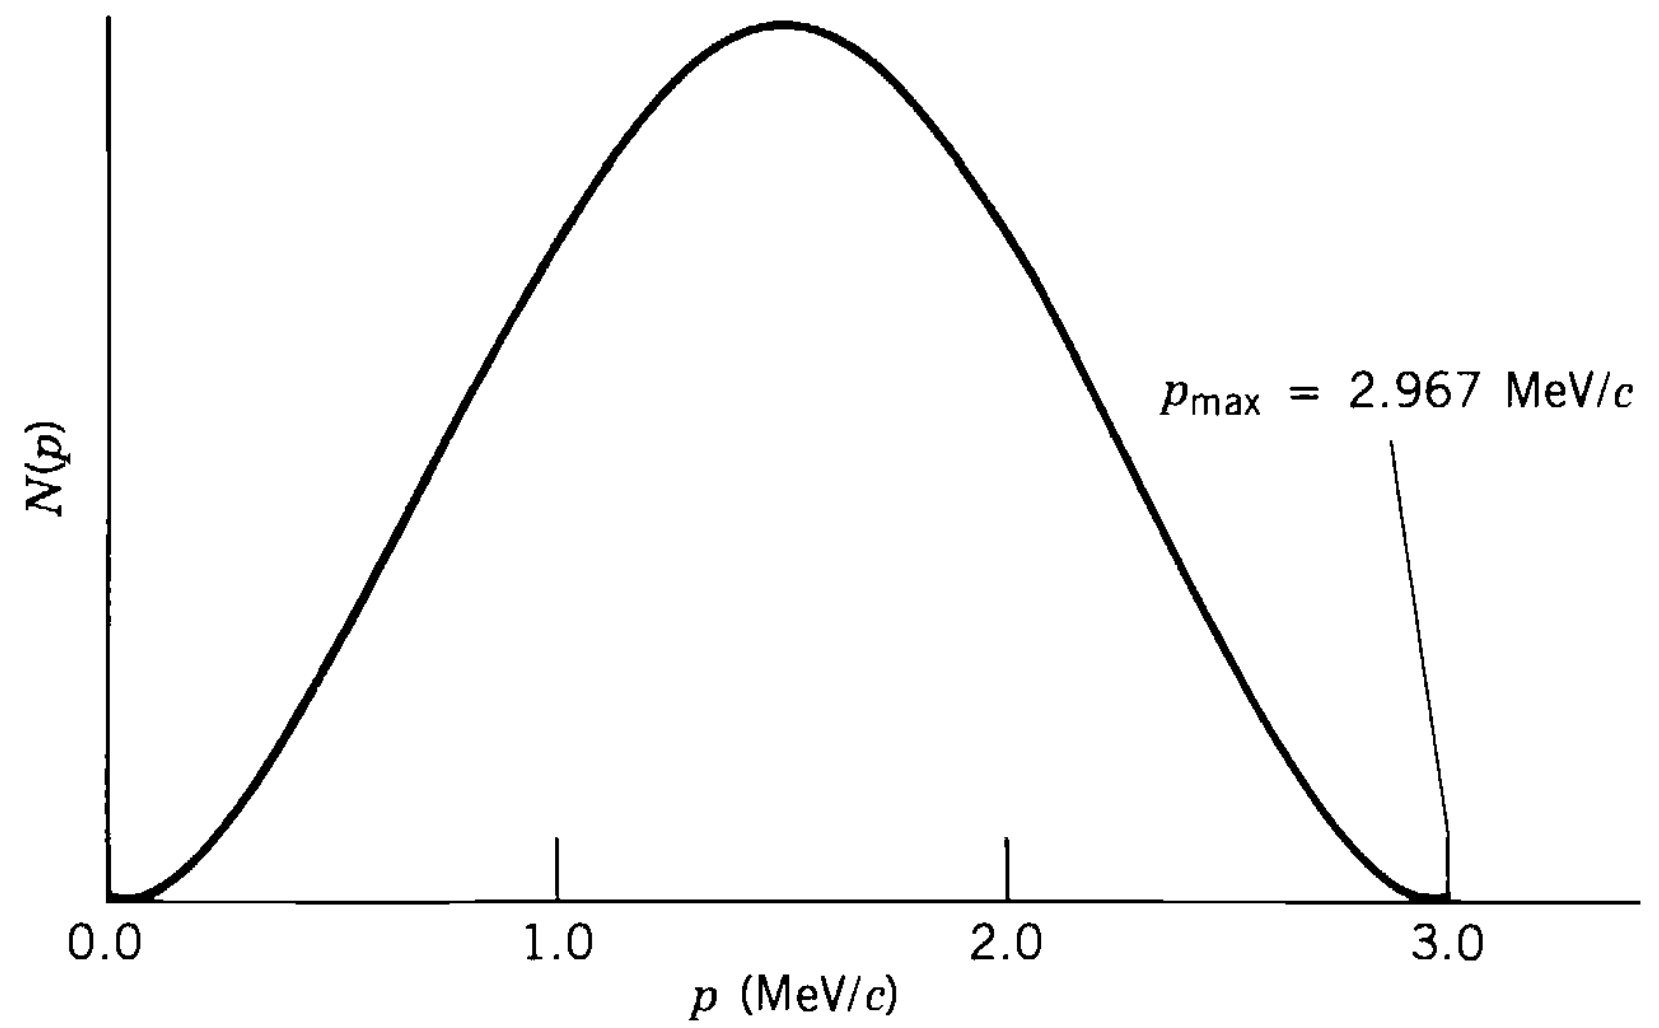
\includegraphics[width=0.45\textwidth]{beta-mom.png}
	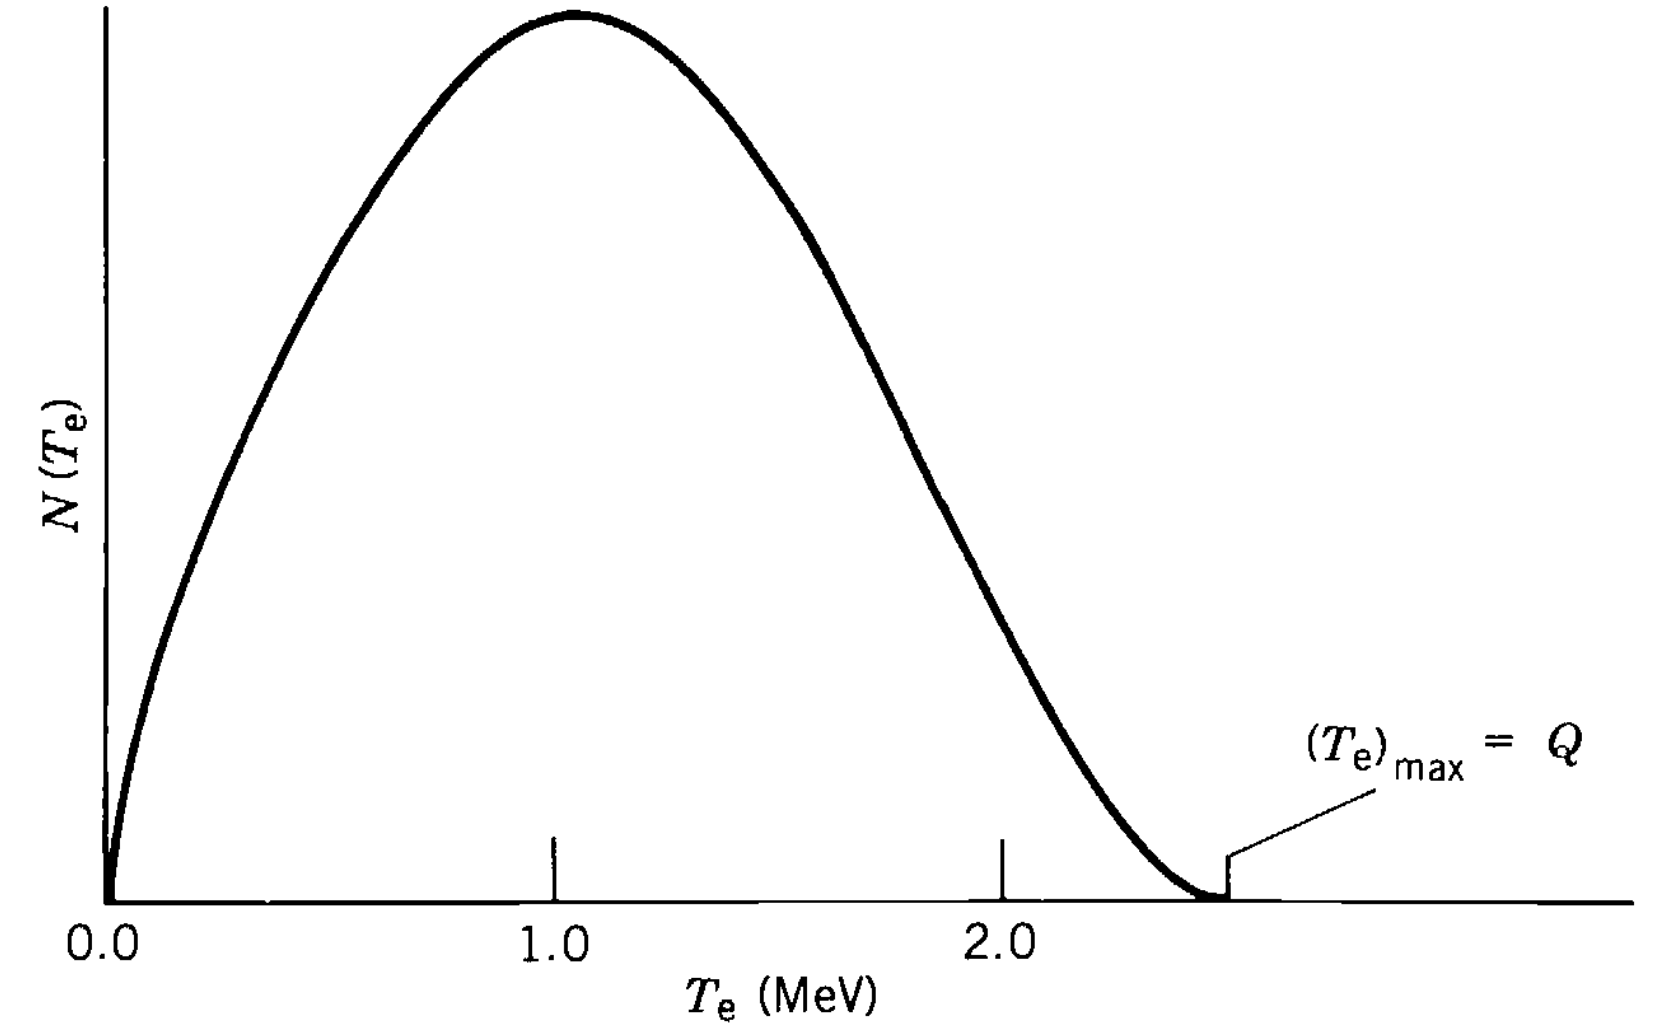
\includegraphics[width=0.45\textwidth]{beta-kin.png}
	\caption{Momentum and energy distributions of electrons from $ \beta $ decay.}
	\label{beta-spectrum}
\end{figure}

Analizzando gli spettri energetici, inoltre, si trova che $ Q_{\beta} \approx Q $: ciò implica che il neutrino ha massa estremamente piccola. Inoltre, per conservazione del momento angolare, è necessario che esso abbia spin semi-intero: considerando ad esempio il decadimento $ \ch{^{14}_6 C} \rightarrow \ch{^{14}_7 N} + e^- + \bar{\nu}_e $, se il neutrino non avesse spin semi-intero si avrebbe una violazione della conservazione di $ I $, dato che entrambi i nuclidi hanno $ I $ intero e l'elettrone ha $ s = \frac{1}{2} $.

\subsection{Teoria di Fermi}\label{fermi-th-sec}

A partire dall'ipotesi del neutrino di Pauli (1931), nel 1934 Fermi formulò una teoria per descrivere il decadimento $ \beta $; in particolare, si fanno le seguenti assunzioni:
\begin{enumerate}
	\item si trascura l'interazione coulombiana tra elettrone e nucleo (valido per nuclei con $ Z < 10 $);
	\item si trascura il nuclear recoil (valido poiché $ m_e \ll M_{\text{nucleo}} $);
	\item si considera il neutrino massless;
	\item si considerano equiprobabili tutte le possibili partizioni dell'energia tra elettrone e neutrino.
\end{enumerate}
Da questi assunti, si ricava che il bilancio energetico del processo è dato da:
\begin{equation}
	E = E_e + E_{\nu} = T_e + m_e c^2 + c p_{\nu}
	\label{eq:2.23}
\end{equation}
dalla quale si trova che $ T_e^{\text{max}} = E - m_e c^2 = Q $. La legge fondamentale postulata da Fermi per descrivere il decadimento è la \textit{golden rule}:
\begin{equation}
	\lambda = \frac{2\pi}{\hbar} \abs{M}^2 \frac{dn}{dE}
	\label{eq:2.24}
\end{equation}
Il termine $ \frac{dn}{dE} $ è dovuto alla natura dello spazio delle fasi e rappresenta la densità degli stati finali possibili per il decadimento ($ dn $ sono gli stati finali energeticamente possibili tra $ E $ ed $ E + dE $), mentre $ \abs{M}^2 $ è detto elemento di matrice dell'operatore di transizione $ \hat{H} $ e stima la probabilità di overlap tra lo stato iniziale e quello finale del sistema:
\begin{equation}
	M \defeq \braket{\psi_{\text{f}} | \hat{H} | \psi_{\text{i}}} = \int_V d^3\ve{x}\, \psi^*_{\text{f}}(\ve{x}) \hat{H} \psi_{\text{i}}(\ve{x})
	\label{eq:2.25}
\end{equation}
dove $ \psi_{\text{f}} = \psi_{\text{Y}} \psi_e \psi_{\nu} $. Il calcolo dell'elemento di matrice è estremamente complicato, specialmente per la difficoltà di calcolare le funzioni d'onda nucleari.\\
Si supponga che nel decadimento l'elettrone venga emesso con momento $ \ve{p}_e $: dato che la direzione di emissione è ininfluente con le semplificazioni fatte, ricordando che l'elemento di volume minimo dello spazio delle fasi è $ h^3 $ si trova che, confinando il sistema in un volume $ V $ (formalità solo per normalizzare le funzioni d'onda), il numero $ dn_e $ di stati elettronici finali con momento tra $ p_e $ e $ p_e + dp_e $ è:
\begin{equation}
	dn_e = \frac{4\pi p_e^2 V}{h^3} dp_e
	\label{eq:2.26}
\end{equation}
Ragionando analogamente per il neutrino, si trova che il numero totale di stati $ dn $ in funzione dei momenti $ p_e $ e $ p_{\nu} $ è:
\begin{equation}
	dn = dn_e dn_{\nu} = \left( \frac{4\pi V}{h^3} \right)^2 p_e^2 dp_e p_{\nu}^2 dp_{\nu}
	\label{eq:2.27}
\end{equation}
Ricordando il vincolo $ E = E_e + E_{\nu} $, si ha che $ cp_{\nu} = E - E_e $ e, fissata $ E_e $, $ dp_{\nu} = \frac{dE}{c} $, quindi:
\begin{equation}
	\frac{dn}{dE} = \left( \frac{4\pi V}{h^3} \right)^2 \frac{1}{c^3} (E - E_e)^2 p_e^2 dp_e
	\label{eq:2.28}
\end{equation}
Si assume $ \abs{M}^2 $ indipendente da $ p_e $, me è necessario considerare una correzione dovuta all'interazione coulombiana a cui è soggetto l'elettrone/positrone: come si vede in Fig. \ref{beta-coul}, la repulsione dei positroni porta ad averne meno ad energie basse, mentre l'attrazione degli elettroni diminuisce quelli ad alta energia. La correzione analitica è data dalla \textit{funzione di Fermi}:
\begin{equation}
	F(Z,E_e) \approx \frac{2\pi \eta}{1 - e^{-2\pi \eta}}
	\label{eq:2.29}
\end{equation}
dove $ \eta $ è il \textit{parametro di Sommerfeld}, che per $ e^{\pm} $ è definito come:
\begin{equation}
	\eta \equiv \mp \frac{Ze^2}{\hbar v_e}
	\label{eq:2.30}
\end{equation}
con $ v_e $ velocità asintotica dell'elettrone/positrone. Per $ \eta \ll 1 $ si ha $ F(Z,E_e) \approx 1 $.\\
È dunque possibile esprimere la probabilità di disintegrazione differenziale grazie alla golden rule:
\begin{equation}
	d\lambda(p_e) = C \abs{M}^2 F(Z,E_e) (E - E_e)^2 p_e^2 dp_e
	\label{eq:2.31}
\end{equation}
con $ C $ una costante. È stato possibile eliminare la dipendenza dal neutrino poiché la sua energia è fissata da quella dell'elettrone/positrone.

\begin{figure}[b!]
	\centering
	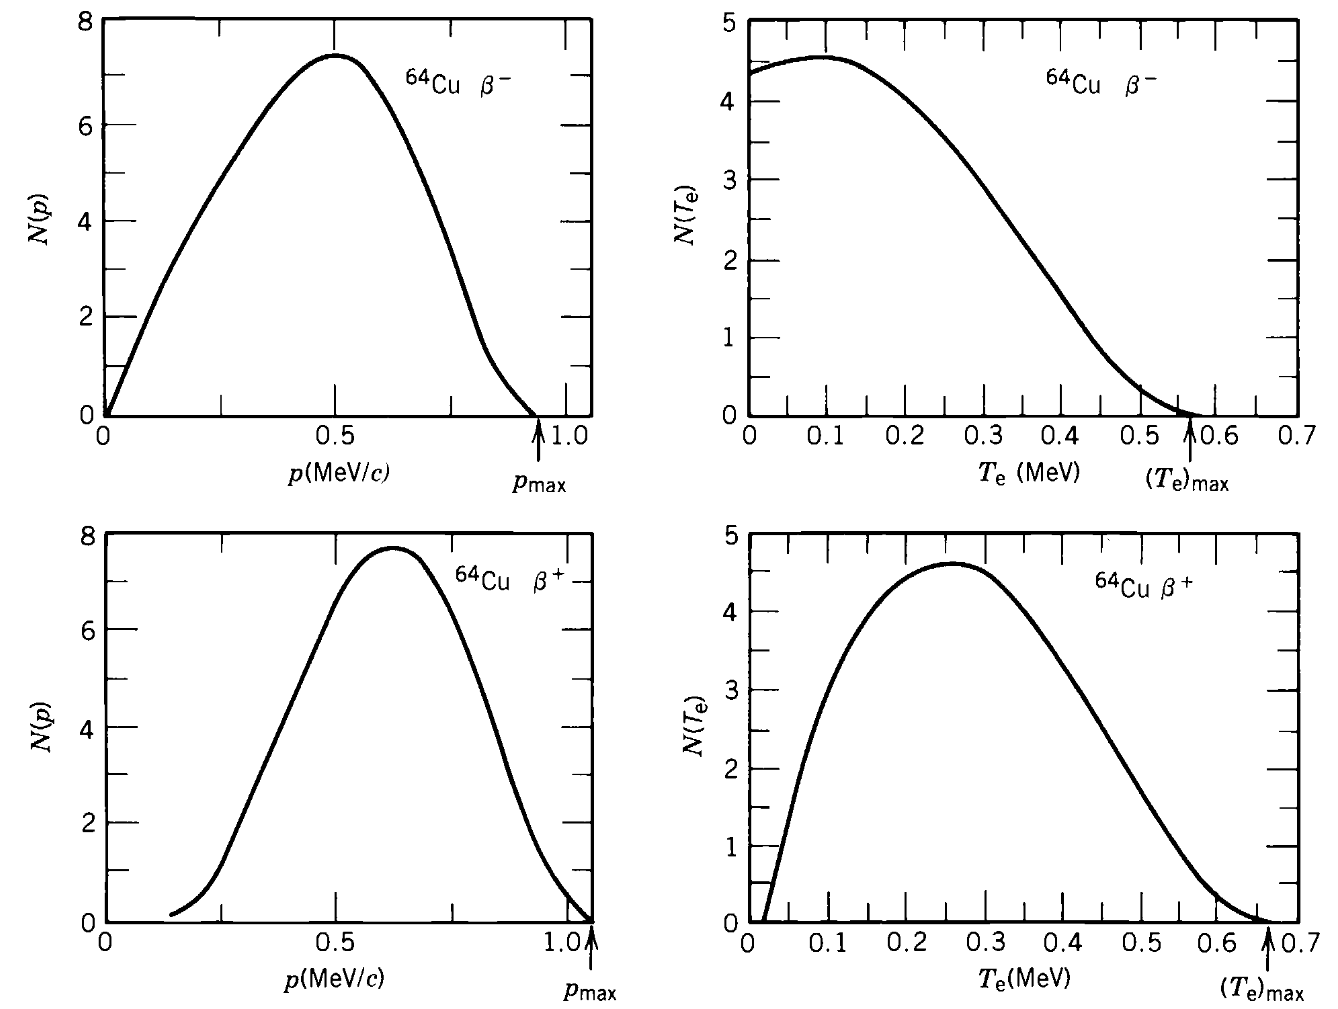
\includegraphics[width=0.70\textwidth]{beta-coul.png}
	\caption{Momentum and kinetic energy spectra of electrons and positrons emitted from $ \ch{^{64}_{29}Cu} $ decay.}
	\label{beta-coul}
\end{figure}

È possibile ottenere $ \lambda $ integrando su $ [0, p_e^{\text{max}}] $, dove il momento elettronico massimo si ottiene ponendo nullo quello neutrinico, ovvero $ p_e^{\text{max}} = \frac{1}{c} \sqrt{E^2 - m_e^2 c^4} $.\\
È inoltre utile definire la \textit{funzione di Fermi-Kurie}:
\begin{equation}
	K(E_e) \defeq \sqrt{\frac{\frac{d\lambda(p_e)}{dp_e}}{p_e^2 F(Z,E_e)}} \propto E - E_e
	\label{eq:2.32}
\end{equation}
Dall'analisi del Fermi-Kurie plot è possibile ottenere informazioni sulla massa del neutrino: infatti, con metodi di regressione lineare è possibile individuare quando $ E - E_e $ si annulla con una buona precisione, mentre misurare in maniera diretta il valore di energia massimo sarebbe complicato.

\subsubsection{Massa del neutrino}

Nel caso in cui si consideri un neutrino di massa non-nulla $ m_{\nu} $, la sua energia va calcolata come:
\begin{equation}
	E_{\nu} = \sqrt{p_{\nu}^2 c^2 + m_{\nu}^2 c^4}
	\label{eq:2.33}
\end{equation}
Differenziando $ p_{\nu}^2 c^2 = (E - E_e)^2 - m_{\nu}^2 c^4 $ e moltiplicando per $ p_{\nu} $, si trova:
\begin{equation}
	p_{\nu}^2 dp_{\nu} = \frac{1}{c^3} \sqrt{(E - E_e)^2 - m_{\nu}^2 c^4} (E - E_e) dE
	\label{eq:2.34}
\end{equation}
Dall'Eq. \ref{eq:2.27}-\ref{eq:2.31}, si trova quindi l'equazione corretta:
\begin{equation}
	d\lambda(p_e) = C \abs{M}^2 F(Z,E_e) \sqrt{(E - E_e)^2 - m_{\nu}^2 c^4} (E - E_e) dE
	\label{eq:2.35}
\end{equation}
Di conseguenza, varia l'andamento di $ K(E_e) $: in particolare, in prossimità di $ E - E_e = 0 $ l'andamento non sarà lineare ma radicale, e diversi valori di $ m_{\nu} $ determineranno end-point energies diverse.\\
Questo è uno dei metodi sperimentali più usati per misurare la massa del neutrino, sebbene nel tempo studi sul decadimento del trizio abbiano portato a risultati diversi: gli ultimi dati dell'esperimento Katrin (Karlsuhe, 2022) pongono $ m_{\nu} < 0.8 \ev $.

\section{Decadimento \texorpdfstring{$ \gamma $}{TEXT}}

Il decadimento $ \gamma $ è un processo elettromagnetico in cui il nucleo diminuisce la sua excitation energy senza variare il numero di protoni e neutroni. Questo decadimento avviene tramite l'emissione di fotoni, i bosoni massless e di spin 1 che mediano l'interazione elettromagnetica, i quali trasportano energie che vanno dai keV alle decine di MeV.\\
Oltre al decadimento $ \gamma $, ci sono altri due modi elettromagnetici di diseccitazione: la pair production, che avviene quando l'emissione di un fotone è proibita dalle selection rules e $ \Delta E > 2m_e = 1.022 \mev $, e l'electron conversion, in cui l'energia da emettere viene ceduta ad un elettrone, il quale viene così emesso dall'atomo (tipicamente elettroni degli orbitali interni). Questi decay modes, però, sono poco probabili, per questo quando si parla di diseccitazione elettromagnetica ci si riferisce sostanzialmente al decadimento $ \gamma $.

\subsection{Caratteristiche del decadimento \texorpdfstring{$ \gamma $}{TEXT}}

Tipicamente il decadimento $ \gamma $ è il decay mode dominante negli stati nucleari eccitati: lo studio dei raggi $ \gamma $ emessi permette di inferire varie proprietà degli stati nucleari coinvolti, come ad esempio lo spin, la parità, il momento magnetico, la vita media etc.\\
Nello studio degli spettri $ \gamma $ bisogna ricordare che è sempre presente un fondo naturale, dovuto al fatto che gli elementi delle principali catene di decadimento (ad esempio quella del $ \ch{^{238}U} $), sebbene decadano $ \alpha $ e $ \beta $, possono venire prodotti non nel loro stato fondamentale ma in uno stato eccitato, dunque prima di proseguire la catena essi decadono $ \gamma $: anche le sorgenti $ \alpha $ e $ \beta $ emettono raggi $ \gamma $.\\
Dato un raggio $ \gamma $ di energia $ E $, ricordando che $ E = h \nu $ e $ \nu \lambda = c $, la sua lunghezza d'onda è:
\begin{equation}
	\lambda = \frac{hc}{E}
	\label{eq:2.36}
\end{equation}
Dunque, un raggio $ \gamma $ di energia $ 1\mev $ (tipico ordine di grandezza) ha una lunghezza d'onda di $ 1240\fm $, ben superiore alle dimensioni del nucleo atomico ($ 6\fm $ per $ A = 100 $).\\
Considerando invece uno stato nucleare eccitato di vita media $ \tau $, dal principio di Heisenberg si può definire la sua \textit{energy width} $ \Gamma $ come:
\begin{equation}
	\Gamma \approx \frac{\hbar}{\tau}
	\label{eq:2.37}
\end{equation}
Per uno stato di vita media $ \tau = 1 \,\text{ps} $ si ha $ \Gamma = 0.66 \cdot 10^{-3} \ev $, che è praticamente infinitesima e trascurabile poiché di vari ordini di grandezza inferiore all'attuale risoluzione dei rilevatori (detector al germanio ha una risoluzione di $ \sim 2\kev $).

\subsubsection{Nuclear recoil}

Si consideri un nuclide di massa $ m $ inizialmente a riposo in uno stato eccitato $ E_0 $: se esso decade in uno stato $ E_1 $ emettendo un raggio $ \gamma $, per la conservazione del momento e dell'energia esso dovrà avere una certa quantità di moto finale $ \ve{p}_r $ di rinculo, determinata da:
\begin{equation*}
	\begin{cases}
		E_0 = E_1 + E_{\gamma} + \frac{p_r^2}{2m} \\
		\ve{0} = \ve{p}_{\gamma} + \ve{p}_r
	\end{cases}
	\quad\Rightarrow\quad p_r = p_{\gamma} = \frac{E_{\gamma}}{c}
\end{equation*}
Il salto energetico $ \Delta E = E_0 - E_1 $ tra i due livelli è dunque:
\begin{equation}
	\Delta E = E_{\gamma} + \frac{E_{\gamma}^2}{2mc^2}
	\label{eq:2.38}
\end{equation}
Per ricavare l'energia del fotone, ricordando che $ \Delta E \ll mc^2 $:
\begin{equation}
	E_{\gamma} = mc^2 \left[ -1 \pm \sqrt{1 + \frac{2\Delta E}{mc^2}} \right] \approx \Delta E - \frac{\Delta E^2}{2mc^2}
	\label{eq:2.39}
\end{equation}
Dato che tipicamente $ \Delta E \sim 1\mev $ e $ mc^2 \sim A \cdot 10^3 \mev $, la correzione dovuta al nuclear recoil è dell'ordine di $ 10^{-5} \Delta E $, dunque in prima approssimazione si può affermare che l'energia del raggio $ \gamma $ è proprio la differenza di energia tra i due stati della transizione:
\begin{equation}
	E_{\gamma} = \Delta E
	\label{eq:2.40}
\end{equation}

\subsection{Emissione di raggi \texorpdfstring{$ \gamma $}{TEXT}}

Un nucleo eccitato emette fotoni quando l'excitation energy non è sufficiente a separare un nucleone dal nucleo (tipicamente servono $ \sim 8\mev $), dunque l'unico modo per diseccitarsi è emettere un fotone (quanto d'energia). Inoltre, ciò può avvenire anche per energie superiori alla soglia di separazione, nel caso in cui l'emissione di nucleone fosse vietata dalle regole di conservazione di parità e/o momento angolare.\\
Dallo studio del pattern di decadimento $ \gamma $ si possono ricavare subito informazioni sulla struttura del nucleo: un pattern regolare indica la presenza di una rotational band, ovvero un nucleo deformato, mentre un pattern irregolare può indicare un nucleo sferico.\\
Il fatto che il nucleo si disecciti tramite emissione di radiazione elettromagnetica si può capire dal fatto che il nucleo è un insieme di cariche che generano un campo elettromagnetico. Si ricordi che la radiazione elettromagnetica può essere generata da una carica oscillante, nel qual caso si parla di \textit{radiazione elettrica} E, o da una corrente/momento magnetico variabile nel tempo, che genera una \textit{radiazione magnetica} M. Inoltre, un campo elettromagnetico variabile generato da cariche e correnti dipendenti dal tempo può essere espresso tramite uno sviluppo in serie di multipoli, ciascuno caratterizzato da una distribuzione angolare di radiazione emessa, che quantisticamente corrispondono ai diversi valori di momento angolare trasportati dal fotone. Dunque, nella descrizione di onde elettromagnetiche, si parla di radiazione di \textit{multipolarità} $ \sigma L $, dove $ \sigma $ può essere E o M, ovvero la natura della radiazione, ed $ L $ è l'ordine di multipolo, ovvero il numero quantico di momento angolare del fotone.\\
A livello nucleare, le varie multipolarità sono dovute a differenti oscillazioni del fluido nucleare: le multipolarità $ \text{E}L $ sono dovute ad una redistribuzione della carica elettrica nel nucleo, mentre quelle $ \text{M}L $ ad una redistribuzione degli spin o dei momenti angolari orbitali dei nucleoni.

\subsubsection{Trattazione semiclassica}

Per studiare la radiazione $ \gamma $ emessa da un nuclide è possibile applicare l'approccio semiclassico, che prevede il calcolo della potenza emessa dai vari ordini multipolari in forma di onde elettromagnetiche: la limitazione di questo approccio è che è valido solo nella \textit{zona di radiazione}, ovvero sviluppando in serie il campo elettromagnetiche ad una distanza molto grande rispetto alle dimensioni della sorgente e alla lunghezza d'onda della radiazione; questa condizione però è sicuramente verificata nel caso del decadimento $ \gamma $. Per una descrizione a qualsiasi distanza è necessario un trattamento completamente quanto-meccanico.\\
In generale, la potenza media (mediata su tutte le direzioni, ovvero su $ \mathbb{S}^2 $) irradiata ad un ordine multipolare $ \sigma L $ è:
\begin{equation}
	P(\sigma L) = \frac{2c}{\epsilon_0} \frac{L + 1}{L [(2L + 1)!!]^2} \left( \frac{\omega}{c} \right)^{2L + 2} \abs{\mathcal{M}(\sigma L)}^2
	\label{eq:2.41}
\end{equation}
dove $ \mathcal{M}(\sigma L) $ è l'elemento di matrice che connette lo stato iniziale a quello finale e che dunque dà la dipendenza dalla struttura nucleare.\\
Per quanto riguarda la distribuzione angolare della radiazione ad un ordine multipolare $ \sigma L $, essa è determinata dal polinomio di Legendre $ P_{2L}(\cos \theta) $: questo rende possibie la determinazione dell'ordine di multipolarità studiando la distribuzione angolare della radiazione. Bisogna inoltre notare che la radiazione elettrica e quella magnetica hanno polarità opposte:
\begin{equation}
	\pi(\text{E}L) = (-1)^{L} \qquad \pi(\text{M}L) = (-1)^{L + 1}
	\label{eq:2.42}
\end{equation}
Ad esempio, la radiazione da dipolo elettrico E1 sarà caratterizzata da:
\begin{equation*}
	P(\text{E}1) = \frac{1}{12\pi \epsilon_0} \frac{\omega^4}{c^3} d^2 \qquad \pi(\text{E}1) = -1
\end{equation*}
dove $ \ve{d} \defeq q\ve{r} $, $ \ve{r} $ vettore di separazione tra le due cariche $ \pm q $. Si vede la parità negativa dal fatto che sotto operatore di parità $ \ve{r} \mapsto -\ve{r} $, dunque $ \ve{d} \mapsto -\ve{d} $.\\
Prendendo invece un dipolo magnetico M1:
\begin{equation*}
	P(\text{M}1) = \frac{1}{12\pi \epsilon_0} \frac{\omega^4}{c^5} \mu^2
\end{equation*}
dove $ \ve{\mu} \defeq q \ve{r}\times\ve{v} $, $ \ve{r} $ posizione e $ \ve{v} $ velocità della carica $ q $ in moto. Sotto operatore di parità $ \ve{r} \mapsto -\ve{r} $ e $ \ve{v} \mapsto -\ve{v} $, dunque $ \ve{\mu} $ rimane invariato.

\subsubsection{Momento angolare}

Dato che il fotone è un bosone di spin 1, esso può sottrarre unità di momento angolare al nucleo in base alla multipolarità della transizione. Dati gli stati iniziale e finale del nuclide, di rispettivo momento angolare $ I_{\text{i}} $ e $ I_{\text{f}} $, dalla conservazione del momento angolare si ottiene la selection rule per il momento angolare $ L $ del raggio $ \gamma $:
\begin{equation}
	\abs{I_{\text{i}} - I_{\text{f}}} \le L \le I_{\text{i}} + I_{\text{f}}
	\label{eq:2.43}
\end{equation}
Dato lo spin 1 del fotone, si ha l'ulteriore vincolo $ L \ge 1 $: di conseguenza, il decadimento $ \gamma $ è proibito per transizioni del tipo $ 0^{\pm} \rightarrow 0^{\pm} $, per i quali sono permesse solo le internal conversions (emissione di un elettrone di conversione) o i decadimenti con più di un fotone (estremamente improbabile). Infatti, la multipolarità E0 (di monopolo) corrisponde ad una distribuzione di carica statica invariante nel tempo, dunque non produce radiazione, mentre M0 non esiste proprio data l'assenza sperimentale di monopoli magnetici.\\
Alcuni nuclidi, come ad esempio $ \ch{^{68}Ni} $, $ \ch{^{90}Zr} $ e $ \ch{^{186}Pb} $, hanno come primo stato eccitato uno stato $ 0^+ $: lo studio di come questi stati decadano al ground state $ 0^+ $ è importante per capire come le diverse forme della superficie nucleare coesistano assieme ad energie simili (dipende da come i nucleoni interagiscono tra loro).

\subsection{Probabilità di transizione}

Data una transizione $ \gamma $ di multipolarità $ \sigma L $, mediata da un fotone di frequenza angolare $ \omega $, si trova la probabilità di transizione come:
\begin{equation}
	T(\sigma L) \equiv \frac{P(\sigma L)}{\hbar \omega} = \frac{2}{\epsilon_0 \hbar} \frac{L + 1}{L [(2L + 1)!!]^2} \left( \frac{\omega}{c} \right)^{2L + 1} B(\sigma L)
	\label{eq:2.44}
\end{equation}
dove si definisce la \textit{probabilità di transizione ridotta} $ B(\sigma L) = \abs{\mathcal{M}_{\text{if}}(\sigma L)}^2 $, indipendente dall'energia di transizione (normalizzato rispetto ad essa) ma dipendente dagli elementi di matrice degli operatori di multipolo tra lo stato iniziale e finale, che è difficile da calcolare dato che non si conoscono con esattezza le funzioni d'onda nucleari.

\subsubsection{Stime di Weisskopf}

Per rendere possibile lo svolgimento analitico del calcolo di $ B(\sigma L) $, si considera il modello a shell (a particelle indipendenti) e si assume che la transizione sia dovuta ad un singolo protone che passa da una shell all'altra: dopo alcune ragionevoli semplificazioni, si ottengono le cosiddette \textit{stime di Weisskopf} per $ B(\sigma L) $.\\
Assumendo una transizione $ \sigma L $ da uno stato eccitato di un nuclide di numero di massa $ A $ al suo ground state:
\begin{equation}
	B(\text{E}L; I_{\text{i}} \rightarrow I_{\text{gs}}) = \frac{(1.2)^{2L}}{4\pi} \left( \frac{3}{L + 3} \right)^2 A^{2L/3} \,e^2 (\text{fm})^{2L}\\
	\label{eq:2.45}
\end{equation}
\begin{equation}
	B(\text{M}L; I_{\text{i}} \rightarrow I_{\text{gs}}) = \frac{10}{\pi} (1.2)^{2L - 2} \left( \frac{3}{L + 3} \right)^2 A^{(2L - 2)/3} \,\mu_N^2 (\text{fm})^{2L - 2}
	\label{eq:2.46}
\end{equation}
Si vede dunque che le probabilità ridotte per transizioni elettriche possono essere espresse in $ e^2 \text{barn}^L $, mentre per transizioni magnetiche in $ \mu_N^2 \text{barn}^{L - 1} $. Queste dipendono dalla multipolarità della transizione, ma non dalla sua energia: la dipendenza da $ E_{\gamma} $ è contenuta nel fattore in Eq. \ref{eq:2.44}. Ad esempio, si trova che $ T(\text{E}1) = 1.0 \cdot 10^{14} A^{2/3} E_{\gamma}^3 $, $ T(\text{E}2) = 7.3 \cdot 10^7 A^{4/3} E_{\gamma}^5 $, $ \dots $, $ T(\text{M}1) = 3.1 \cdot 10^{13} E_{\gamma}^3 $, $ T(\text{M}2) = 2.2 \cdot 10^7 A^{2/3} E_{\gamma}^5 $, $ \dots $\\
Si trova che, in generale, confrontando tra transizioni dello stesso tipo (E o M), la probabilità di transizione $ T $ diminuisce all'aumentare di $ L $, anche di 4 ordini di grandezza, mentre a parità di ordine di multipolo sono predominanti le transizioni elettriche, di 2 o 3 ordini di grandezza.\\
$ T(\sigma L) $ è espresso in $ \text{s}^{-1} $ e può essere identificato nella costante di decadimento $ \lambda $ della transizioni $ \sigma L $; di conseguenza, si ha che la vita media dello stato eccitato è $ \tau = \frac{1}{T(\sigma L)} $: queste variano da $ 10^{-15}\,\text{s} $ a svariati anni, tempi estremamente grandi rispetto al tempo medio in cui un nucleone attraversa il nucleo ($ \sim 10^{-22}\,\text{s} $). Inoltre, se le uniche transizioni ammesse dalle selection rule tra due stati sono ad alto ordine multipolare, la vita media può essere talmente lunga (giorni o anni, mentre tipicamente è $ \sim 1\text{ps} $) che si parla di \textit{stati isomerici}.\\
Il confronto dei valori teorici di Weisskopf con i dati sperimentali è molto importante: una probabilità di transizione molto pià piccola del previsto può indicare che i due stati nucleari iniziale e finale sono molto diversi tra loro, mentre una probabilità molto più grande del previsto può equivalere al fatto che nella transizione sono coinvolti non uno a molti nucleoni. Il confronto avviene esprimendo le probabilità osservate sperimentalmente in Weisskopf units $ B_{\text{sp}} $, ovvero studiando il rapporto $ B(\sigma L) / B_{\text{sp}}(\sigma L) $: questo si attesta circa all'unità nell'intorno delle double shell closures, a riprova che le stime teoriche descrivono bene i nuclei caratterizzati dalle eccitazioni di nucleoni singoli, mentre può assumere valori anche di qualche centinaia per nuclei in cui si hanno stati collettivi, ad esempio quelli caratterizzati da stati vibrazionali di quadrupolo nei nuclidi sferici o nelle rotational bands dei nuclidi deformati.










